\newif\iffunny
\funnyfalse

\documentclass[xcolor={dvipsnames}]{beamer}
\usepackage{color, colortbl}
\usepackage[ngerman,english]{babel}
\usepackage[T1]{fontenc}
\usepackage{CJKutf8} %japanese
\usepackage{lmodern}
%\usepackage{subfigure}
\usepackage[compatibility=false]{caption}
\usepackage{subcaption}
\usepackage{tikz}
\usepackage{textgreek}
\usepackage{tabularx}
\usepackage{booktabs}
\usepackage{siunitx}
\usepackage{units}
\usepackage{appendixnumberbeamer}
\usepackage[absolute,overlay]{textpos} %for positioning the logos where I want

\usepackage{animate}
\usepackage{multimedia}
\usepackage{fixltx2e}
\usepackage{multicol}
\usepackage{comment}
\DeclareSIUnit\year{yr}

\mode<presentation>
{
  \usetheme{CambridgeUS}     
  \usecolortheme{lily} 
  \definecolor{beamer@violet}{rgb}{0.5,0.3,0.5} % changed this
  \setbeamercolor{structure}{fg=beamer@violet!70!cyan}
  \setbeamercolor{palette primary}{fg=black, bg=gray!30!white!50!cyan!20!}
  \setbeamercolor{palette secondary}{fg=black, bg=gray!30!white!30!cyan!40!}
  \setbeamercolor*{palette tertiary}{bg=gray!20!white!20!cyan!60!}
  
  \setbeamercolor{frametitle}{fg=cyan!60!white!40!,bg=cyan!80!black}
  \setbeamercolor{title}{fg=cyan!80!black}
  \setbeamercolor{normal text}{fg=black,bg=white}
  \setbeamercolor{alerted text}{fg=beamer@violet}
  \setbeamercolor{example text}{fg=beamer@violet!70!cyan}
  
  \usefonttheme{structureitalicserif} 
  \setbeamertemplate{navigation symbols}{}
  \setbeamertemplate{caption}[numbered]
}
\newcommand{\sidlogo}{
  \setlength{\TPHorizModule}{1pt}
  \setlength{\TPVertModule}{1pt}
   % textblock{}{x,y}: pos(x) = rightUpperCorner + (x * \TPHorizModule), pos(y) = leftUpperCorner - (y * \TPVertModule)
  \begin{textblock}{1}(323,12)
   
\includegraphics[width=40pt,height=26pt]{figures/SiD.jpeg}
  \end{textblock}
  } 
\newcommand{\ilclogo}{
  \setlength{\TPHorizModule}{1pt}
  \setlength{\TPVertModule}{1pt}
   % textblock{}{x,y}: pos(x) = rightUpperCorner + (x * \TPHorizModule), pos(y) = leftUpperCorner - (y * \TPVertModule)
  \begin{textblock}{1}(323,12)
   
\includegraphics[width=40pt,height=26pt]{figures/ILC.jpeg}
  \end{textblock}
} 
\newcommand{\ejadelogo}{
  \setlength{\TPHorizModule}{1pt}
  \setlength{\TPVertModule}{1pt}
   % textblock{}{x,y}: pos(x) = rightUpperCorner + (x * \TPHorizModule), pos(y) = leftUpperCorner - (y * \TPVertModule)
  \begin{textblock}{1}(323,12)
   
\includegraphics[width=40pt,height=26pt]{figures/EJADE.jpeg}
  \end{textblock}
} 
\newcommand{\ATFlogo}{
  \setlength{\TPHorizModule}{1pt}
  \setlength{\TPVertModule}{1pt}
   % textblock{}{x,y}: pos(x) = rightUpperCorner + (x * \TPHorizModule), pos(y) = leftUpperCorner - (y * \TPVertModule)
  \begin{textblock}{1}(323,12)
   
\includegraphics[width=40pt,height=26pt]{figures/ATF_logo.jpg}
  \end{textblock}
} 
\newcommand{\RHULlogo}{
  \setlength{\TPHorizModule}{1pt}
  \setlength{\TPVertModule}{1pt}
   % textblock{}{x,y}: pos(x) = rightUpperCorner + (x * \TPHorizModule), pos(y) = leftUpperCorner - (y * \TPVertModule)
  \begin{textblock}{1}(337,12)
   
\includegraphics[width=25pt,height=26pt]{figures/rhul_logo.png}
  \end{textblock}
}
\newcommand{\flukalogo}{
  \setlength{\TPHorizModule}{1pt}
  \setlength{\TPVertModule}{1pt}
   % textblock{}{x,y}: pos(x) = rightUpperCorner + (x * \TPHorizModule), pos(y) = leftUpperCorner - (y * \TPVertModule)
  \begin{textblock}{1}(315,12)
   
\includegraphics[width=60pt,height=26pt]{figures/fluka_logo.png}
  \end{textblock}
} 

\newcommand{\electron}{e$^-$}
\newcommand{\positron}{e$^+$}

\title[ILC \& Background Simulations]{\textbf{\LARGE The International Linear Collider \\ \normalsize- \\ \small Background Simulations \& Optimizing the Final Focus Region}}
\author{\textbf{Anne Sch\"utz}}
\institute{\textbf{KIT, DESY}}
\date{\textbf{March 23rd 2016}}

\titlegraphic{
\includegraphics[height=1.0cm]{figures/KIT.png}\hspace*{6cm}~%
   
\includegraphics[height=1.2cm]{figures/DESY_Logo.png}
}

\begin{document}

{
\usebackgroundtemplate{
 \tikz\node[opacity=0.1]{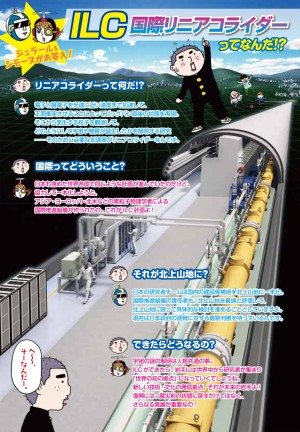
\includegraphics[width=\paperwidth]{figures/Iwatecomics.jpg}};
 % \tikz\node[opacity=0.2]{\centering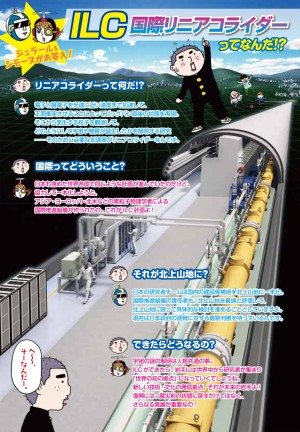
\includegraphics[height=\paperheight]{figures/Iwatecomics.jpg}};
 }
\begin{frame}
  \titlepage
\end{frame}
}

\begin{frame}{Table of contents}
\begin{multicols}{2}
  \tableofcontents
\end{multicols}
\end{frame}

\AtBeginSubsection[]
{
  \begin{frame}<beamer>
     \tableofcontents[currentsection,
     currentsubsection,
     %hideothersubsections,
     subsectionstyle=show/shaded/hide]
  \end{frame}
}

\section{My Ph.D topic and myself}
\subsection{About me}

\begin{frame}{About me}
\begin{columns}
\begin{column}[T]{0.6\textwidth}
Anne Sch\"utz\\
\begin{itemize}
\item Studied Physics at KIT
\item Master's Thesis at DESY: \\ \textit{Simulating the Particles Fluxes at the DESY-II Test Beam Facility}
\item Since April 2015: Ph.D Thesis at DESY
\end{itemize}
\vspace*{0.7cm}
My supervisors\\
\begin{itemize}
\item Prof. Dr. G\"unter Quast (KIT)
\item Prof. Dr. Eckhard Elsen (CERN)
\item Dr. Marcel Stanitzki (DESY)
\end{itemize}
\end{column}

\begin{column}[T]{0.35\textwidth}
\vspace{0pt}%
\centering
	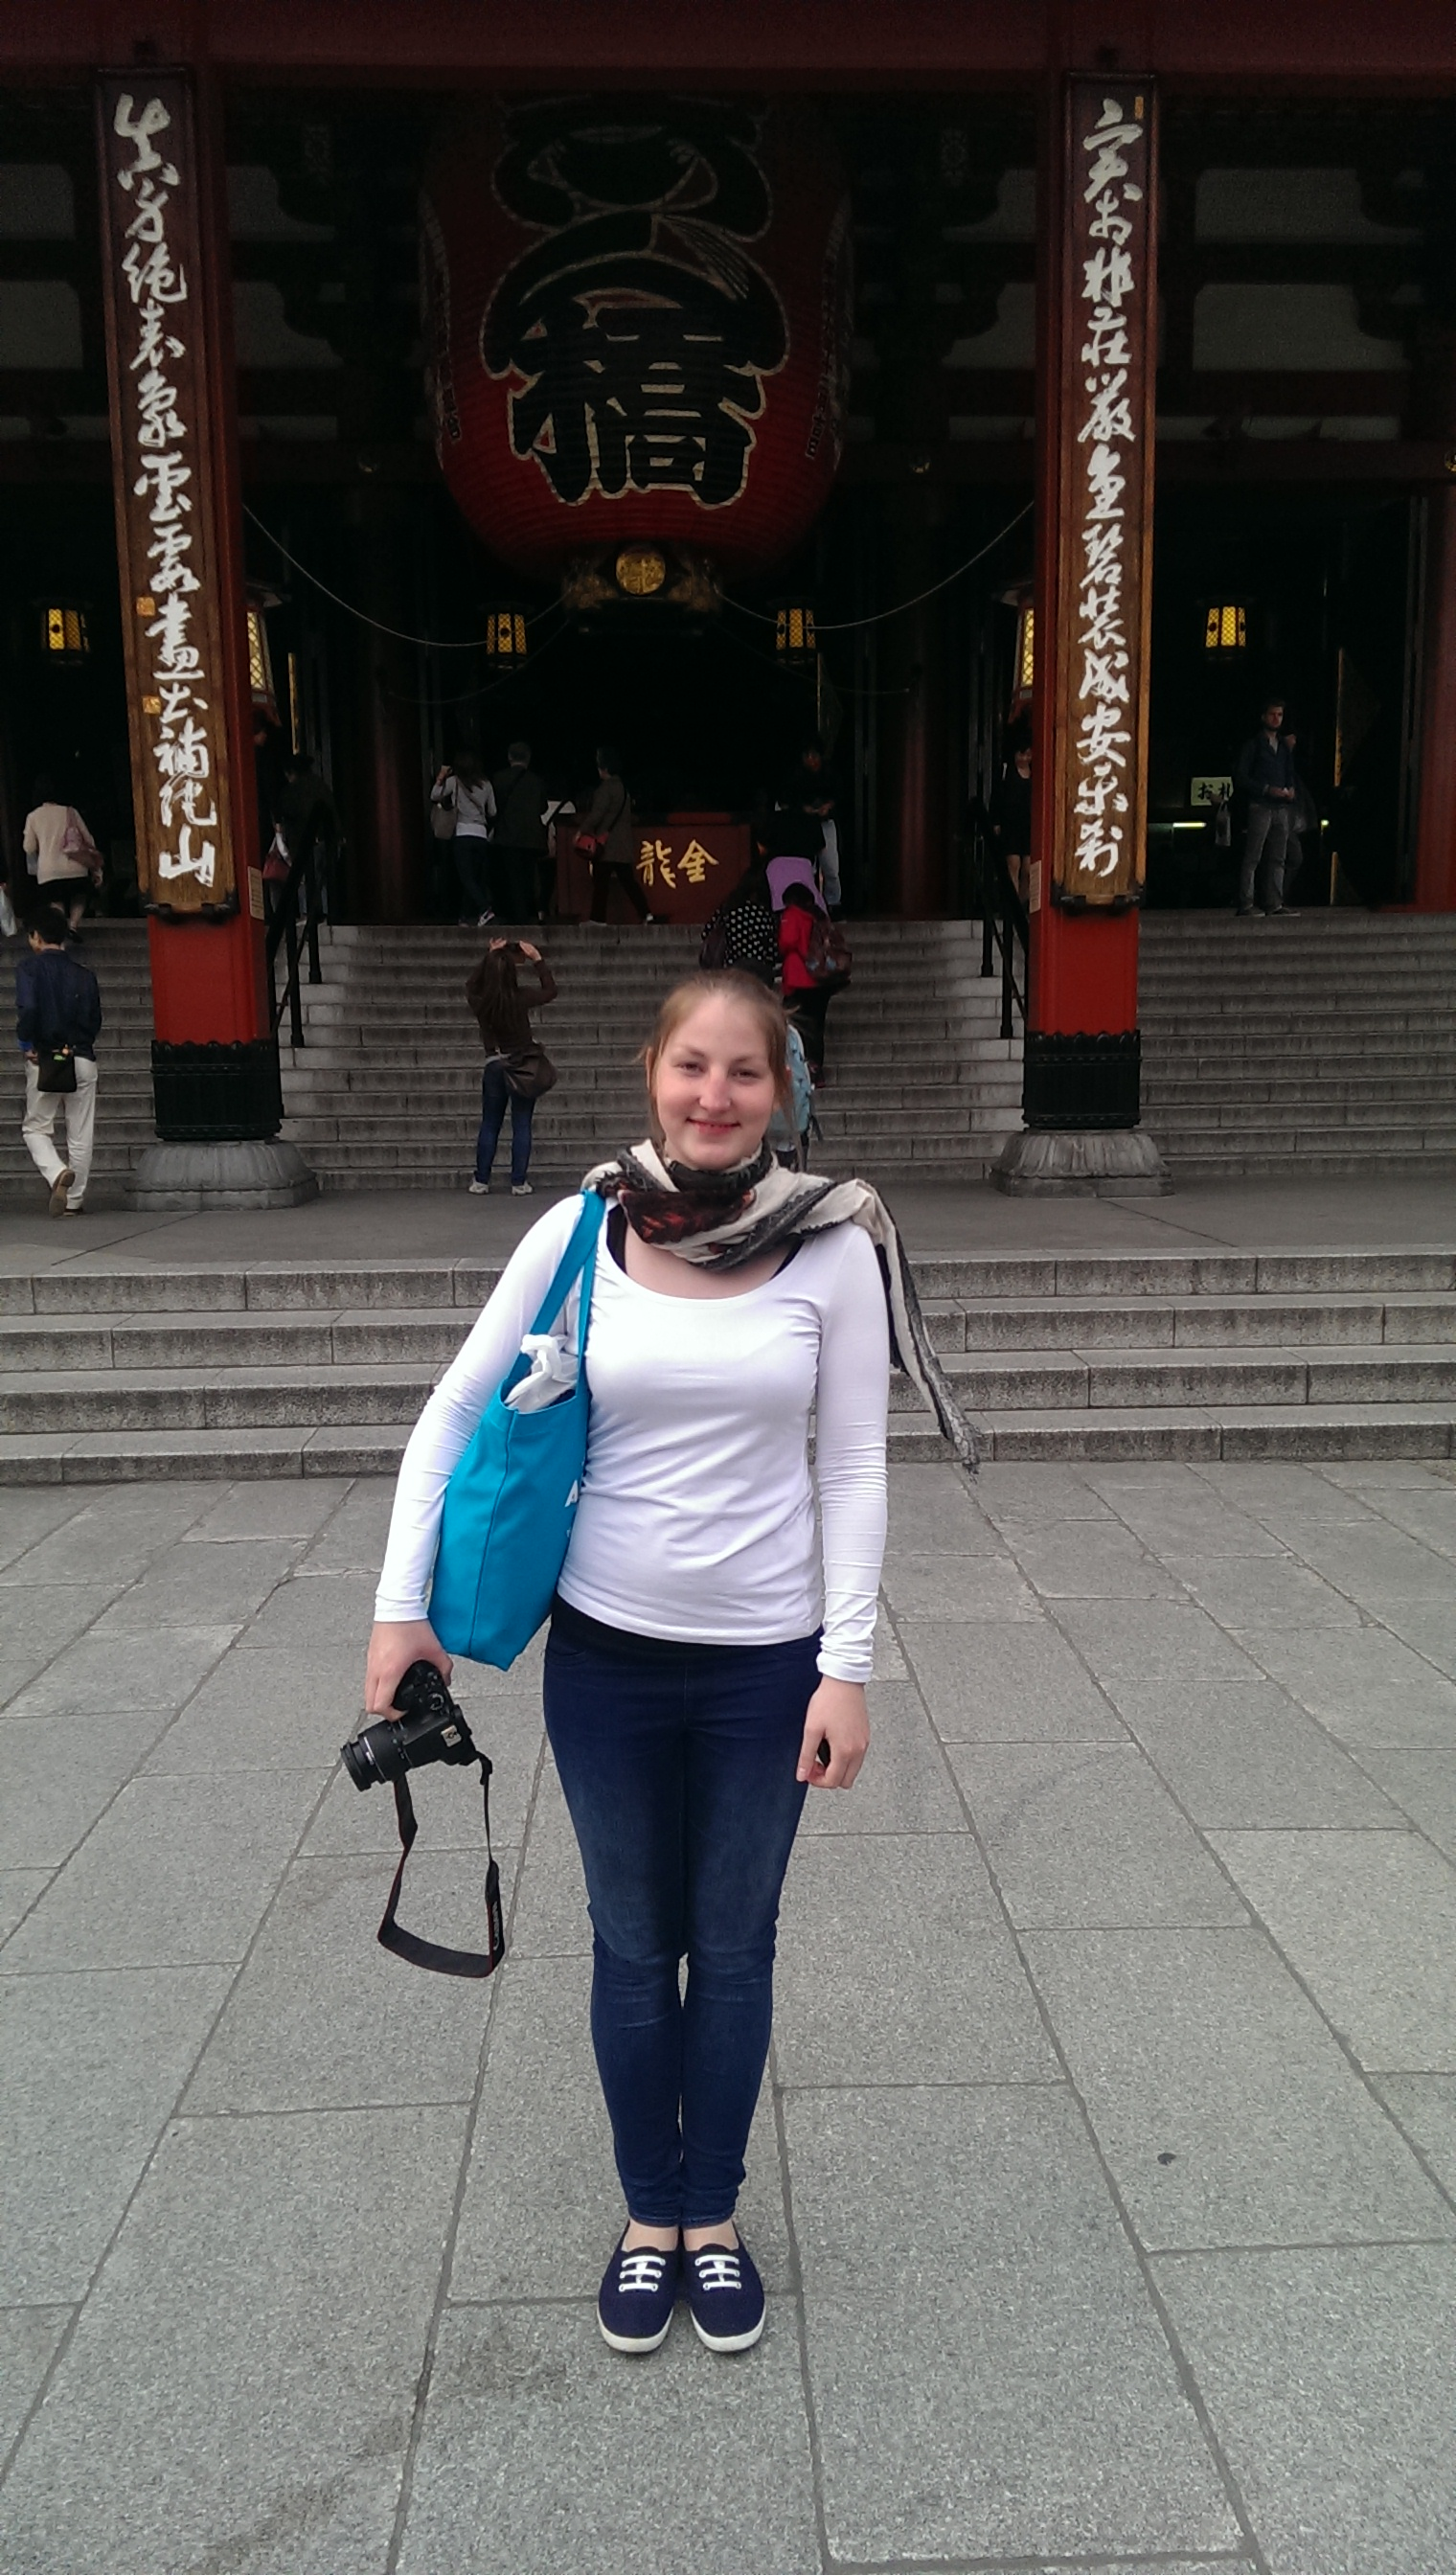
\includegraphics[width=0.7\textwidth]{figures/Myself_inJapan.jpg}
\end{column}
\end{columns}

\end{frame}

\subsection{My Ph.D topic}
\begin{frame}{My Ph.D topic}
\ilclogo
\begin{center}
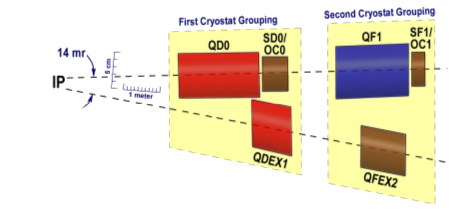
\includegraphics[width=0.4\textwidth]{figures/ILCTDR-VOLUME_3-PART_II_FFRegion.png}
\begin{block}{}
\centering
\textit{Optimizing the design of the Final-Focus Region\\for the International Linear Collider}
\end{block}
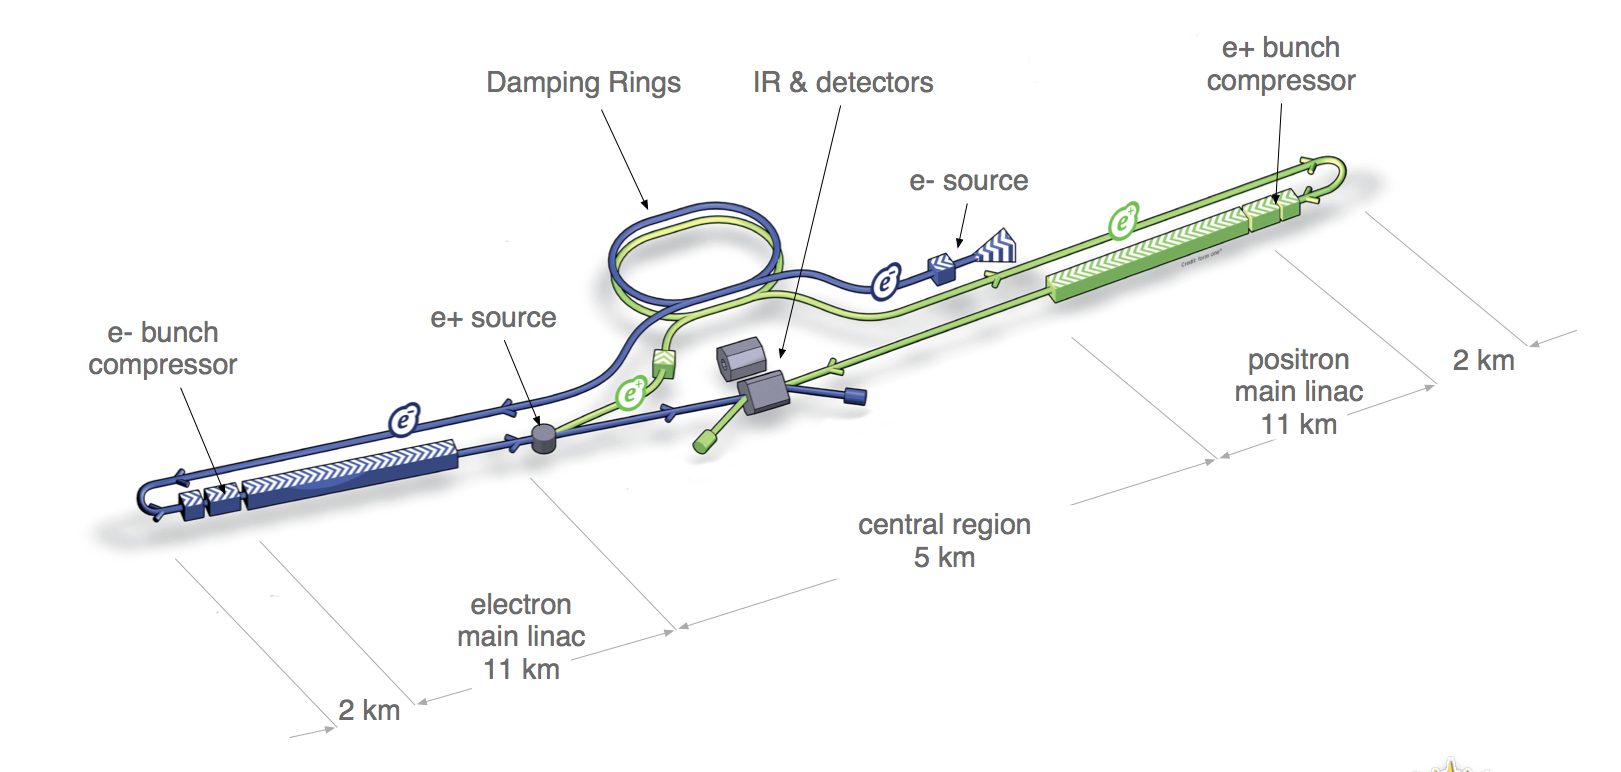
\includegraphics[width=0.7\textwidth]{figures/ILC_schematic_layout.png}
\end{center}
\end{frame}

\section{The International Linear Collider}

\subsection{The layout}
\begin{frame}{The layout of the ILC}
\ilclogo

e$^+$e$^-$ linear collider with adjustable center-of-mass energy, and polarized beams\\
\begin{center}
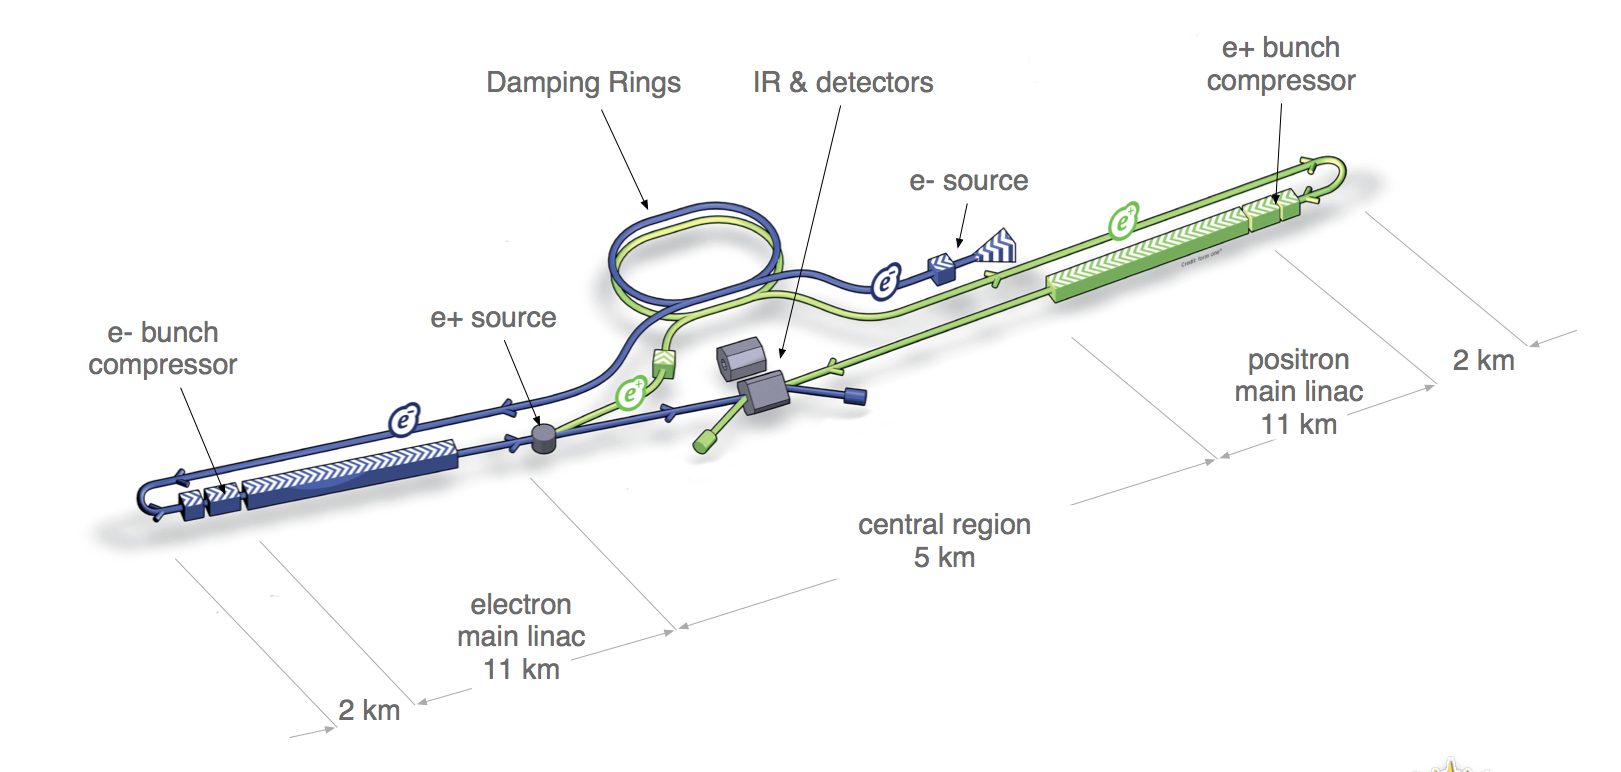
\includegraphics[width=\textwidth]{figures/ILC_schematic_layout.png}
\end{center}
\begin{flushright}
 \href{https://www.youtube.com/watch?v=ep5496vdEFI}{\beamergotobutton{\begin{CJK}{UTF8}{min}国際リニアコライダー\end{CJK}}}
\end{flushright}

\end{frame}

\begin{frame}{Why linear?}
\begin{columns}
 \begin{column}{0.6\textwidth}
  Basic limitations of lepton synchrotons:
\begin{itemize}
 \item \textcolor{Red}{Energy loss due to synchrotron radiation: $\sim$ E$^4$/R}
 \item \textcolor{Red}{Cost $\sim$ quadratically with energy}\\ \tiny{(B. Richter 
1980)}
\end{itemize}
\vspace*{1cm}
Therefore a linear collider:
\begin{itemize}
 \item \textcolor{ForestGreen}{Not limited by synchrotron radiation}
 \item \textcolor{ForestGreen}{Cost $\sim$ linear with energy}
\end{itemize}
 \end{column}
 \begin{column}{0.4\textwidth}
 \begin{block}{}
  \begin{center}
      \textcolor{Gray}{P$_S=\frac{e^2c}{6\pi\epsilon_0}\frac{1}{(m_0c^2)^4}\frac{E^4}{R^2}$\\
  $\Delta$E$=\frac{e}{3\epsilon_0(m_0c^2)^4}\frac{E^4}{R}$}
   \end{center}
 \end{block}
 \end{column}
\end{columns}

\end{frame}

\subsection{The candidate site of the ILC}
\begin{frame}{The candidate site - The Kitakami mountains}
\ilclogo
\begin{center}
\begin{minipage}[t]{0.49\textwidth}
\centering
 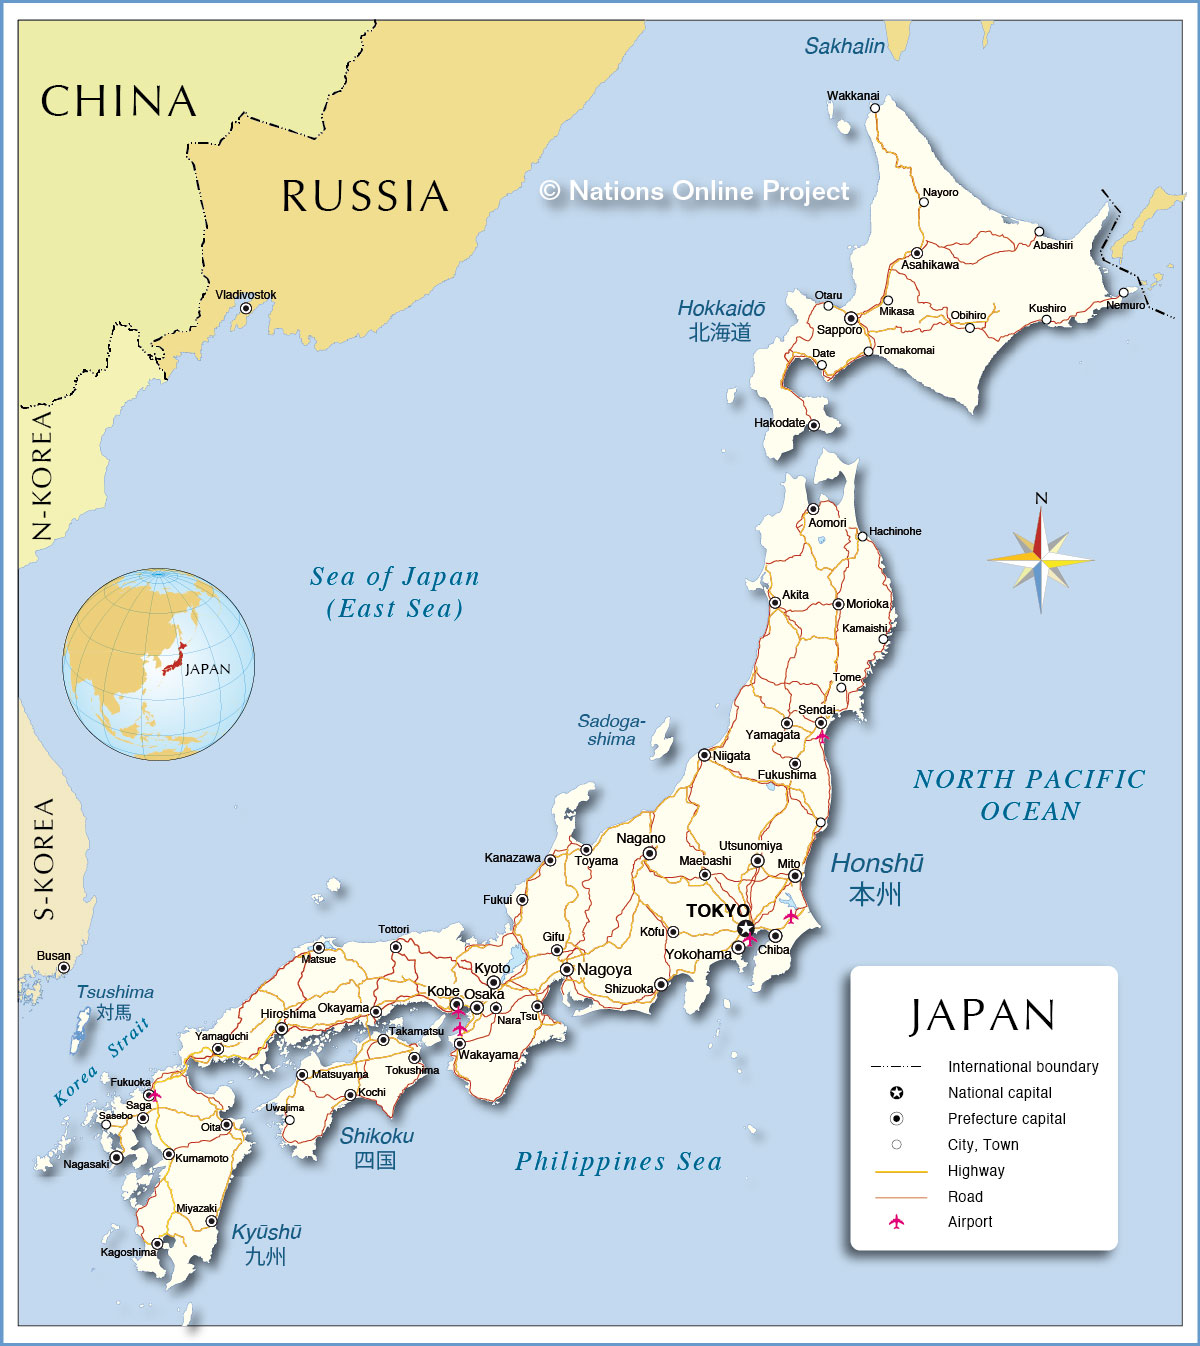
\includegraphics[width=\textwidth]{figures/japan-map.jpg}
\end{minipage}
\begin{minipage}[t]{0.48\textwidth}
\centering
   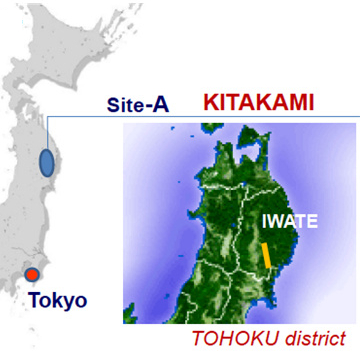
\includegraphics[width=\textwidth]{figures/Kitakami_site.jpg}
\end{minipage}
\end{center}
\end{frame}



%------Definition for column color in table
\definecolor{Gray}{gray}{0.9}
\newcolumntype{g}{>{\columncolor{Gray}}r}
%-----------------------------------------
\subsection{The beam parameters}
\begin{frame}{The beam parameters of the ILC}
\ilclogo

\begin{table}[]
\centering
\begin{tabularx}{\textwidth}{ll|rrrg}
\hline
& & \multicolumn{1}{>{\centering}p{1.5cm}}{\textbf{Baseline 500}} & \multicolumn{1}{>{\centering}p{1.5cm}}{\textbf{Lumi Upgrade}} & \multicolumn{1}{>{\centering}p{1.5cm}}{\textbf{TeV Upgrade}} & {\centering\textbf{LHC 25ns}} \\ 
\hline
\cline{1-6}
\hline
E$_{CM}$  &[\si{\GeV}] & 500  & 500  & \num{1000} & \num{14000}\\
n$_b$ & & \num{1312} & \num{2625} & \num{2450} &  \num{2808} \\
$\Delta t_b$ &[\si{\nano\second}] & 554  & 366   & 366 & 25 \\
N & & \num{2.0e10}  & \num{2.0e10}  & \num{1.74e10}  & \num{11.5e10}\\
q$_b$ &[\si{\nano\coulomb}] & 3.2  & 3.2  &  2.7 & 18.4 \\
$\sigma_x^*$ &[\si{\nano\metre}] & 474  & 474  &  481 & \num{16700}\\
$\sigma_y^*$ &[\si{\nano\metre}] & 5.9 &  5.9  &  2.8 & \num{16700}\\
$\sigma_z$ &[\si{\milli\metre}] & 0.3  &  0.3  &  0.25 & 0.755\\
L &[\si{\per\centi\metre\squared\per\second}] & \num{1.8e34} & \num{3.6e34} & \num{3.6e34} & \num{1.0e34}\\
\hline
\end{tabularx}
\end{table}
\end{frame}

\subsection{The detectors}
\begin{frame}{The two detectors - SiD and ILD}
\ilclogo
\begin{block}{}
The ILC has only one Interaction Point (IP).\\
The two detectors can be swapped in the so-called \textbf{push-pull-system}.
\end{block}

\begin{columns}
\begin{column}{0.48\textwidth}
\begin{center}
\alert{SiD - Silicon Detector}
\begin{itemize}
\item Height: $\sim$\SI{14}{\metre}, length:  $\sim$\SI{11}{\metre}
\item Weight: $\sim$\SI{10100}{\tonne}
\item Superconducting solenoid field: \SI{5}{\tesla}
\item Full silicon tracker
\end{itemize}

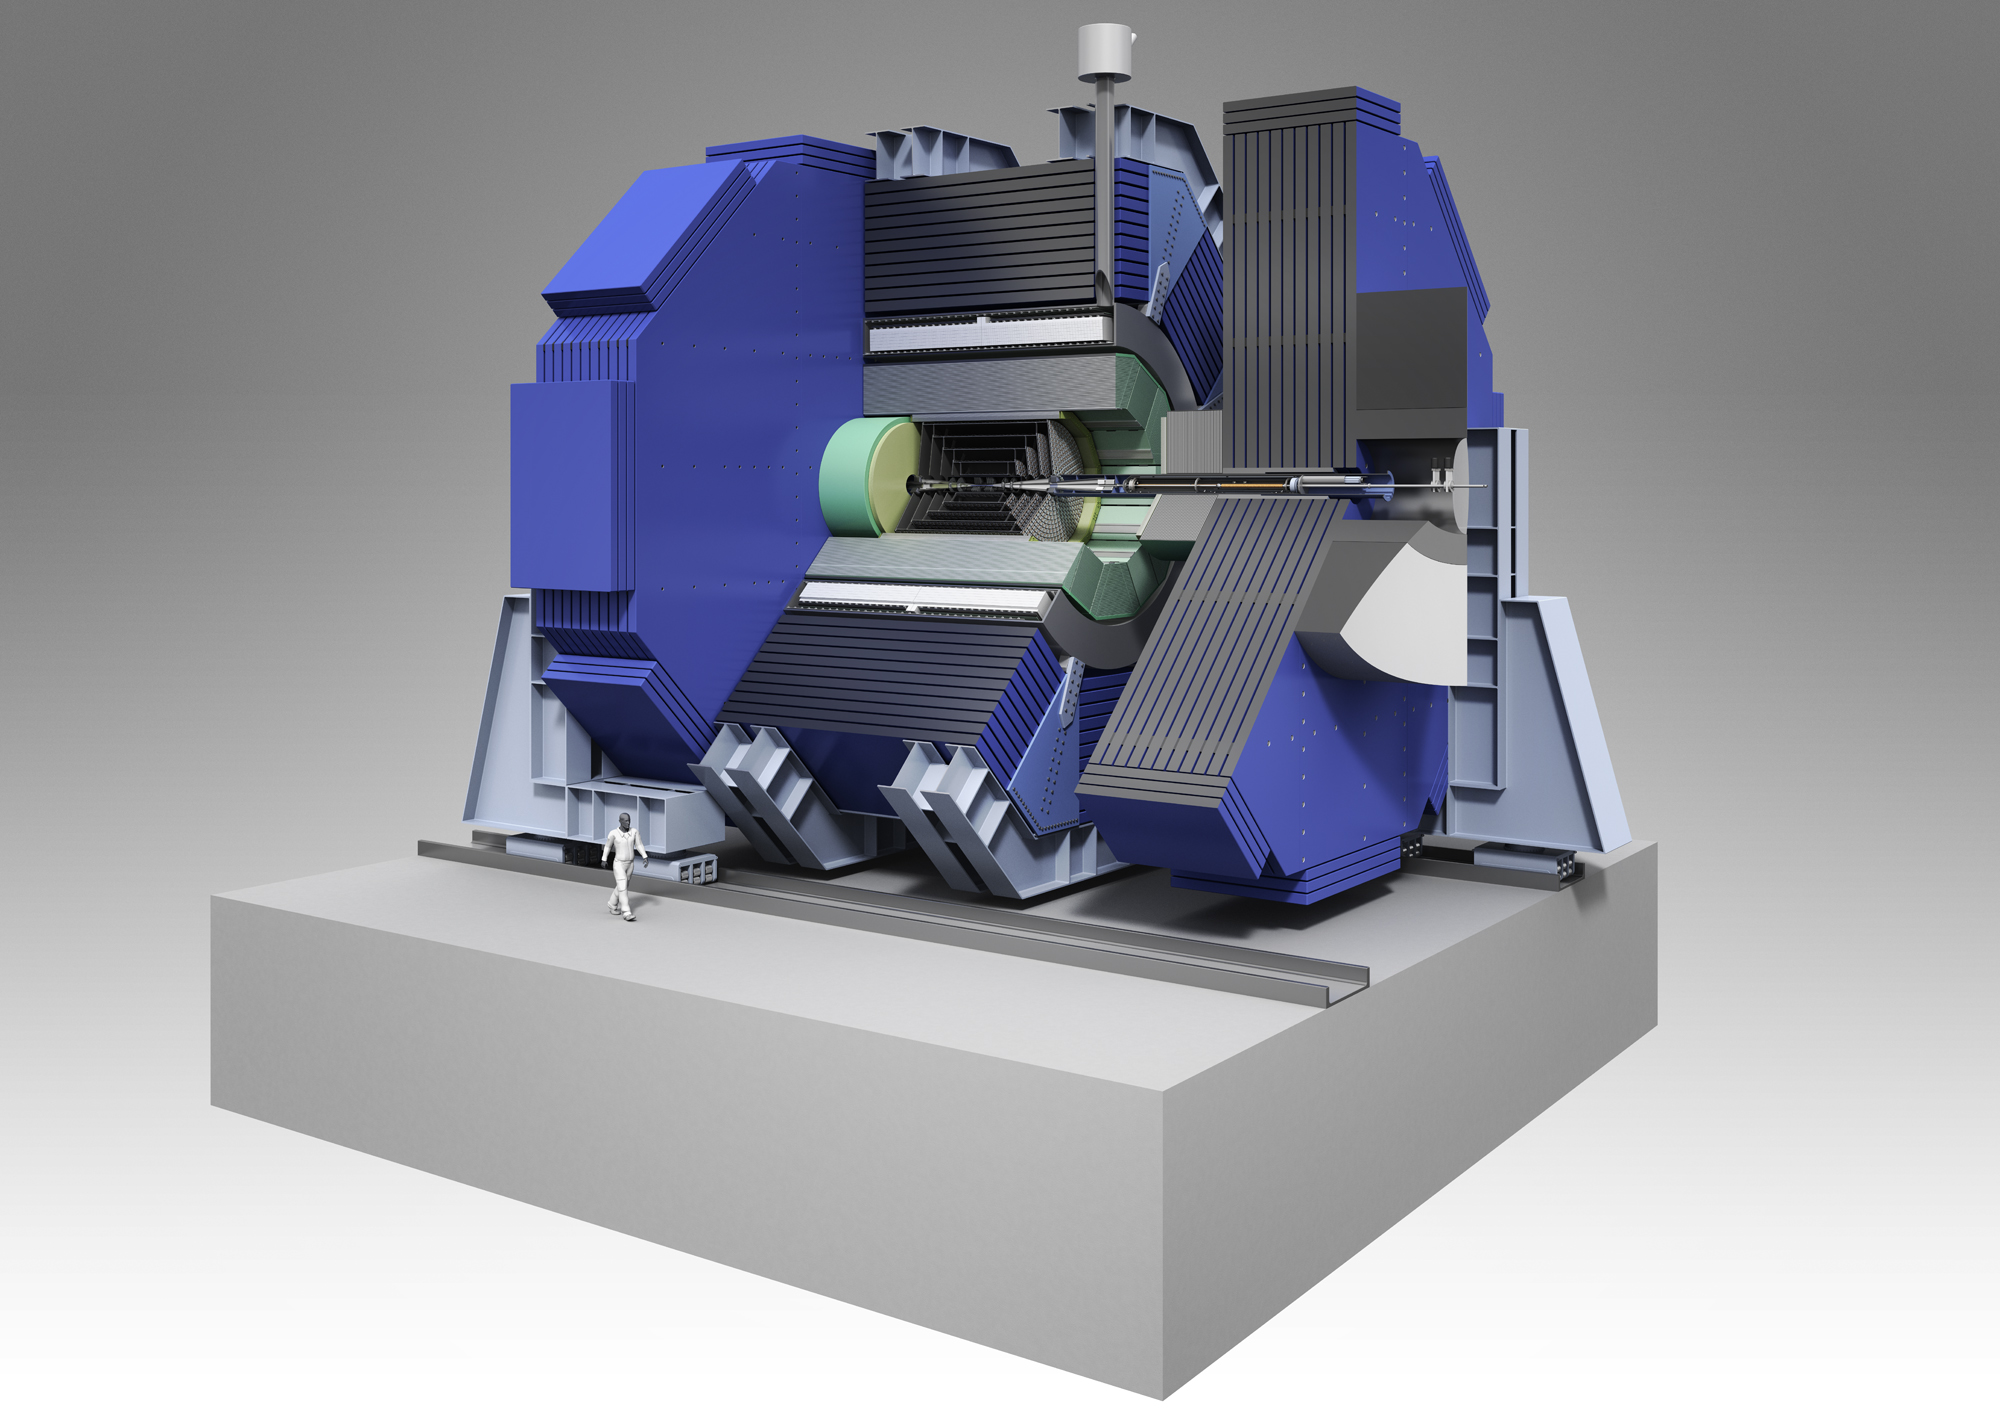
\includegraphics[width=0.5\textwidth]{figures/SiDmodel.jpg}

\end{center}
\end{column}

\begin{column}{0.48\textwidth}
\begin{center}
\alert{ILD - International Large Detector}
\begin{itemize}
\item Height: $\sim$\SI{16}{\metre}, length:  $\sim$\SI{14}{\metre}
\item Weight: $\sim$\SI{14000}{\tonne}
\item Superconducting solenoid field: \SI{3.5}{\tesla}
\item TPC
\end{itemize}

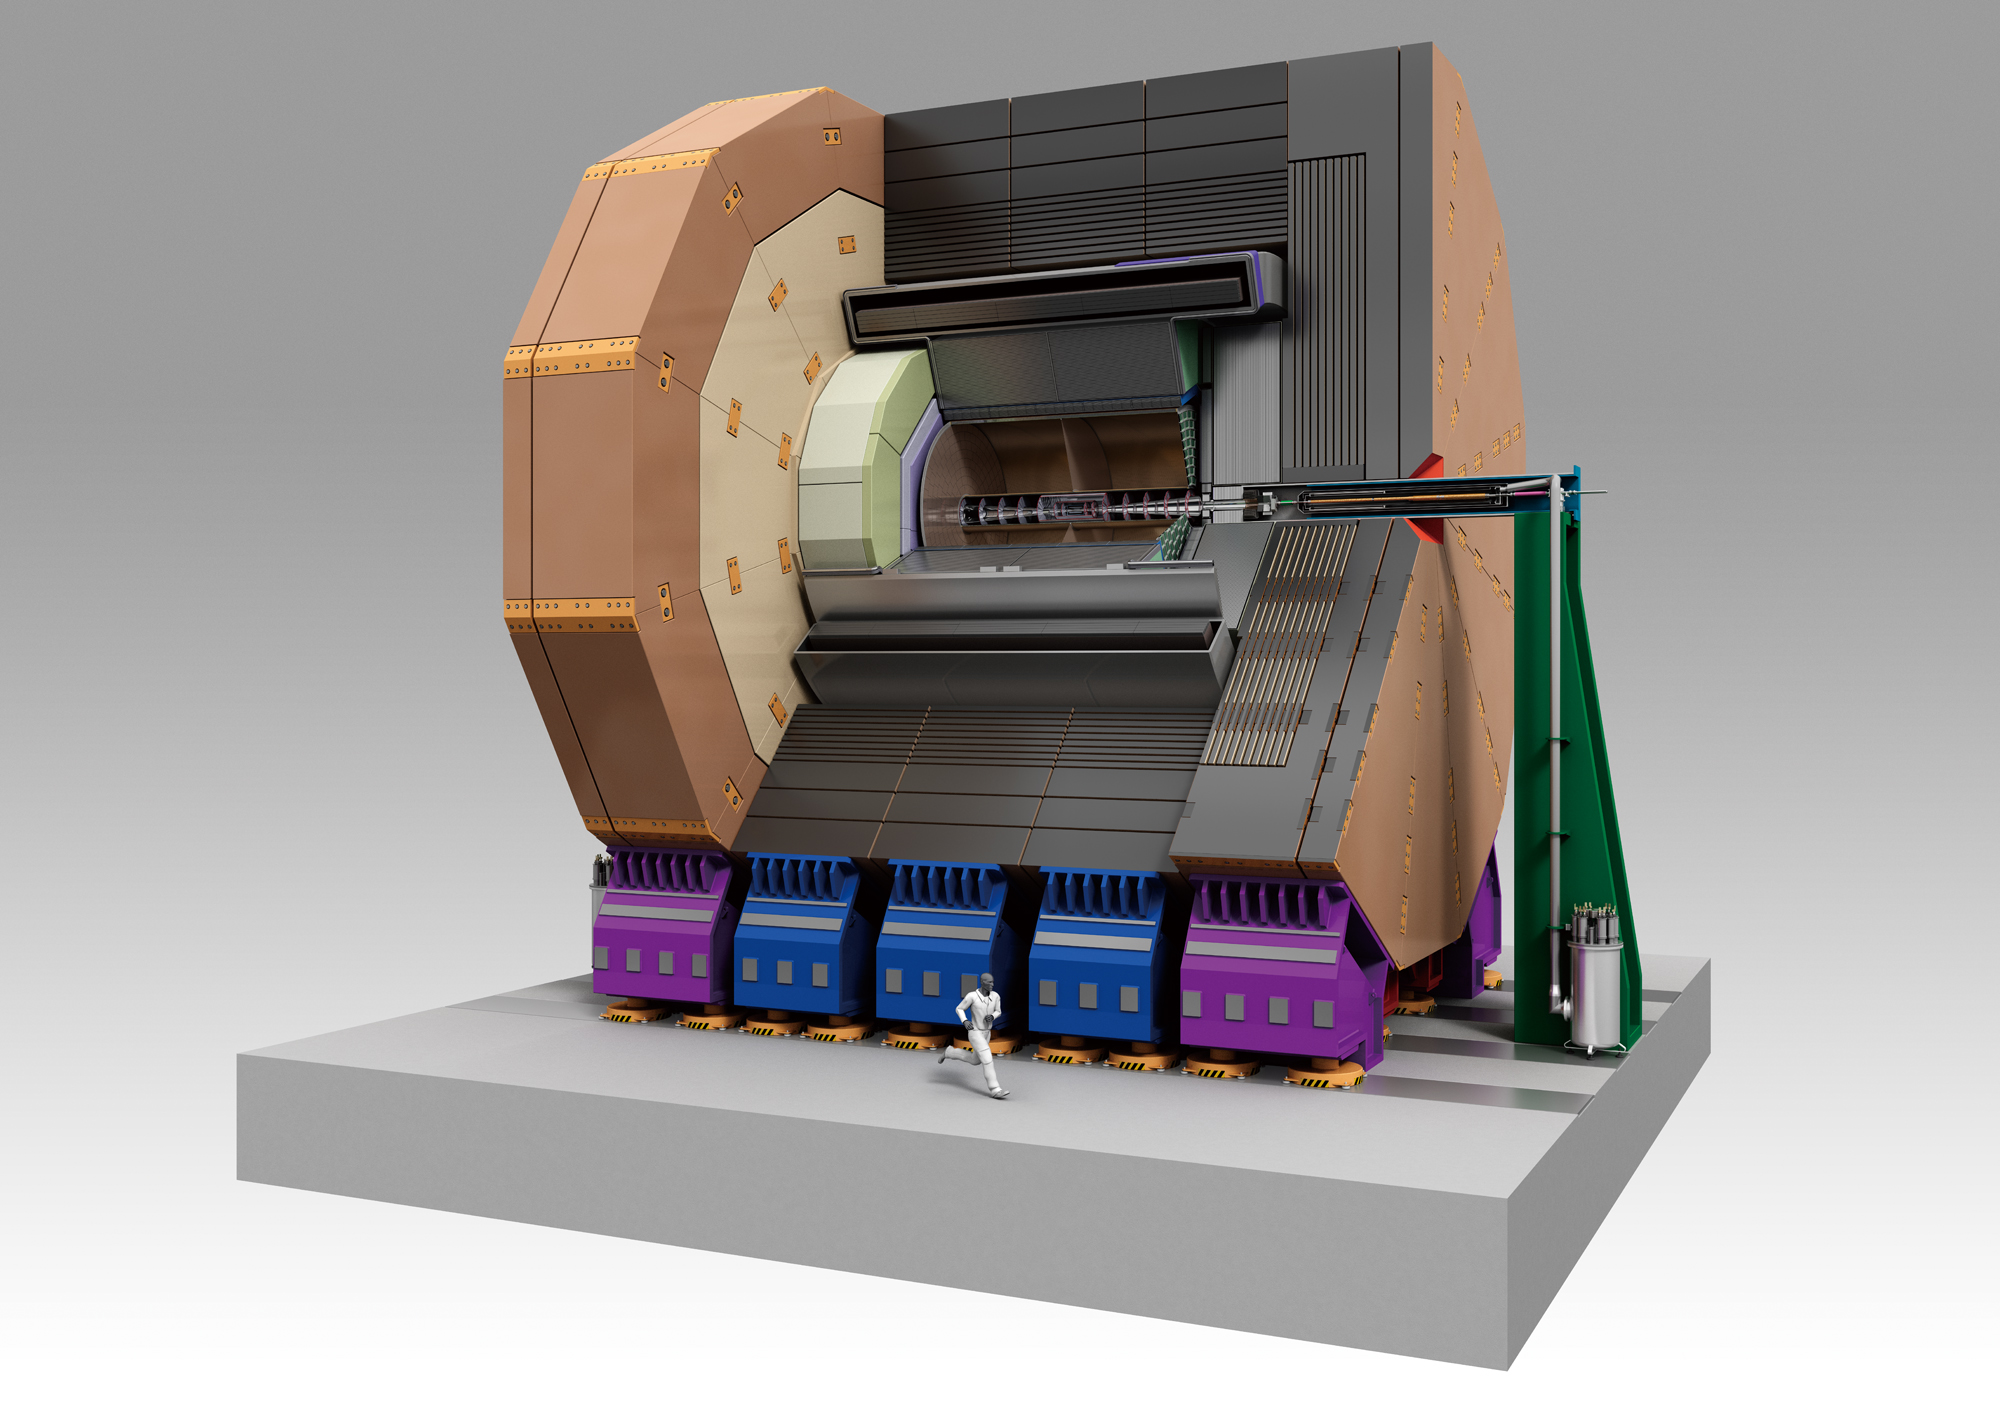
\includegraphics[width=0.5\textwidth]{figures/ILDmodel.jpg}

\end{center}
\end{column}
\end{columns}

\end{frame}
%--------------------------------------------------------------
\subsection{Physics motivation}
\begin{frame}[fragile]{The physics motivation of the ILC}
\ilclogo

\begin{block}{}
\centering
\textcolor{JungleGreen}{Cleanliness} - \textcolor{WildStrawberry}{Democracy} - \textcolor{Periwinkle}{Calculability} - \textcolor{LimeGreen}{Detail}
\end{block}

\visible<2->{
\begin{overprint}
\onslide<2>
\begin{itemize}
\color{JungleGreen}
\item Small background
\item Small detector occupancy
\item Smaller energy range
\item No out-of-time pileup or underlying events
\end{itemize}
\centering
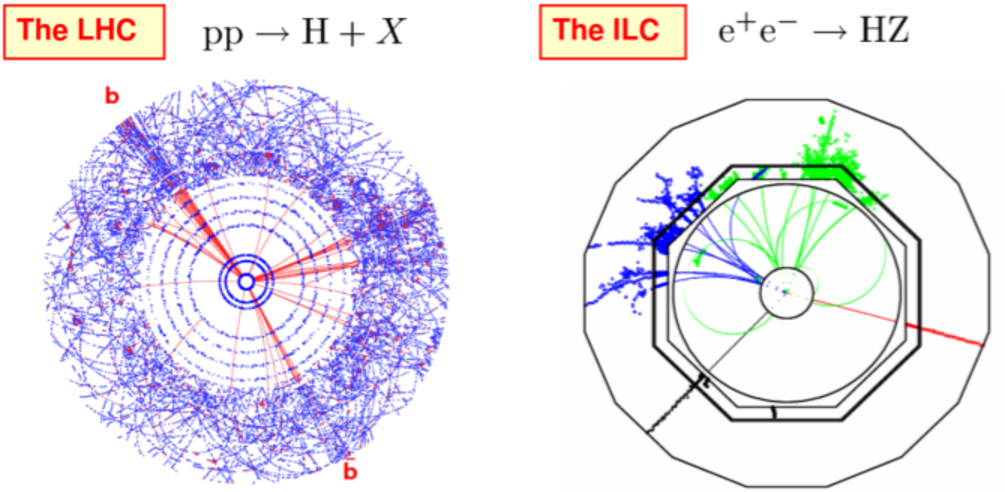
\includegraphics[width=0.6\textwidth]{figures/ILC_LHC_eventdisplay_comparison.pdf}

\onslide<3>
\begin{itemize}
\color{WildStrawberry}
\item Elementary coupling \textit{e} of photons is the same for all quarks and leptons
\item e$^+$e$^-$ annihilation produces pairs of all species, SM and exotics, at similar rates
\item No triggers
\end{itemize}

\onslide<4>
\begin{itemize}
\color{Periwinkle}
\item Point-like elementary particles in initial state
\item Coupling only to electroweak interactions
\item No systematic uncertainties due to PDF uncertainties and QCD corrections
\end{itemize}

\onslide<5>
\begin{itemize}
\color{LimeGreen}
\item Reconstruction of complete events
\item Quark and lepton momenta determined by kinematic fits
\item Study of spin-dependence of production and decay processes
\end{itemize}

\onslide<6>
\begin{columns}
\begin{column}{0.24\textwidth}
\begin{itemize}
\color{JungleGreen}
\item Small background
\item Small detector occupancy
\item Smaller energy range
\item No out-of-time pileup or underlying events
\end{itemize}
\end{column}
\begin{column}{0.26\textwidth}
\begin{itemize}
\color{WildStrawberry}
\item Elementary coupling \textit{e} of \textgamma \, the same for all quarks \& leptons
\item e$^+$e$^-$ annihilation produces pairs of all species, SM \& exotics, at similar rates
\item No triggers
\end{itemize}
\end{column}
\begin{column}{0.27\textwidth}
\begin{itemize}
\color{Periwinkle}
\item Pointlike elementary particles in initial state
\item Coupling only to EW interactions
\item No sys. uncert. due to PDF uncertainties and QCD corrections
\end{itemize}
\end{column}
\begin{column}{0.27\textwidth}
\begin{itemize}
\color{LimeGreen}
\item Reconstruction of complete events
\item Quark \& lepton momenta determined by kinematic fits
\item Study of spin-dependence of production \& decay process
\end{itemize}
\end{column}
\end{columns}
\end{overprint}
}%end visible
\end{frame}

\begin{comment}
\begin{frame}{The physics motivation of the ILC - Higgs factory}
\ilclogo
\begin{itemize}
\item Higgs factory\\
Fraction of the total cross section for Higgs production:\\
In pp: \num{e-9}, in e$^+$e$^-$: \num{e-2} $\approx$ 1\%
\item Each individual Higgs coupling will be measured to a percent accuracy, and the global width of the Higgs can be measured directly:\\LHC experiments have to make a global fit to all Higgs signals (plus using theoretical assumptions of the width), in order to get the Higgs couplings $ \rightarrow$ can never be as precise as at the ILC
\end{itemize}
\visible<2->{
\begin{columns}
 \begin{column}[t]{0.5\textwidth}
   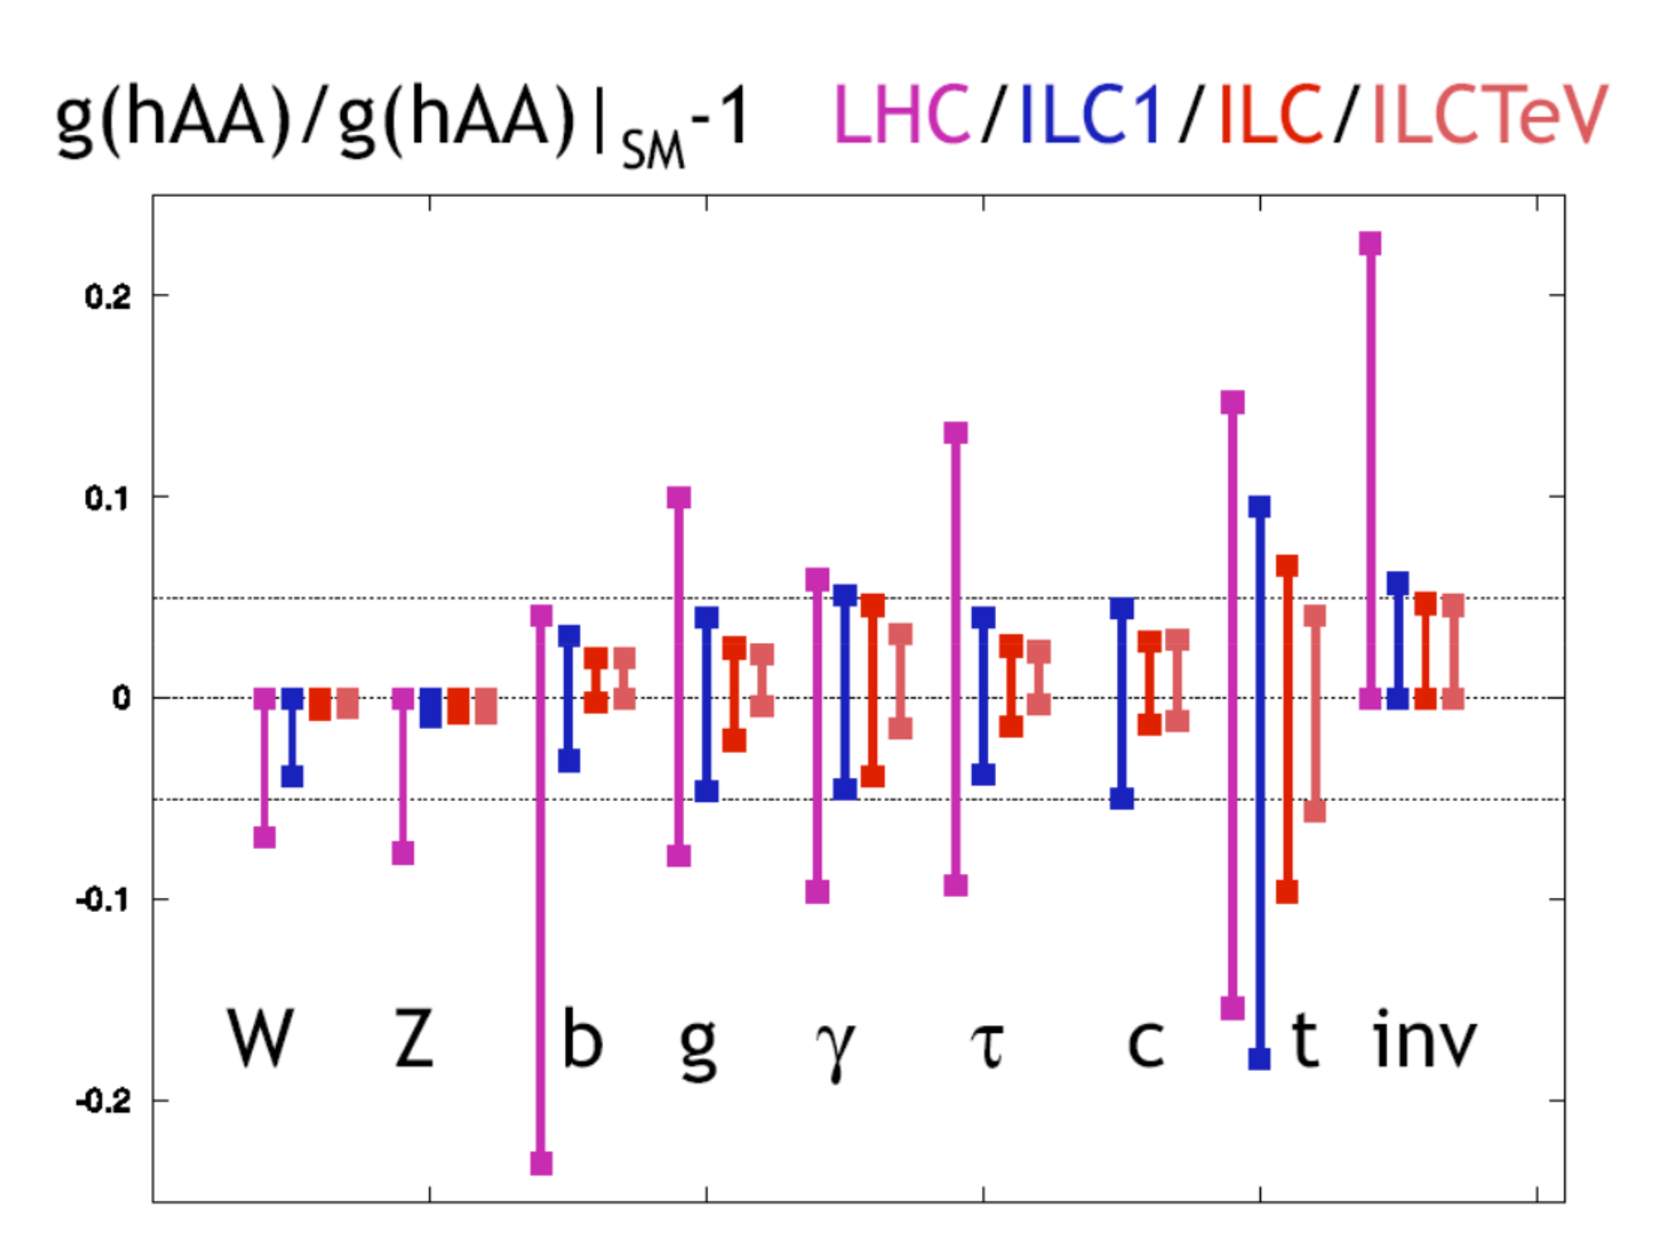
\includegraphics[width=0.85\textwidth]{figures/PhysicsMotivation-ILCPAC2012-Peskin_PrecisionHiggsCouplings.pdf}
 \end{column}
 \begin{column}[t]{0.5\textwidth}
   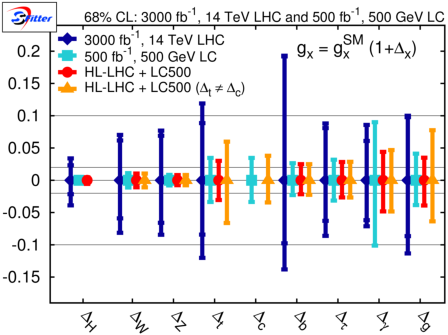
\includegraphics[width=0.83\textwidth]{figures/Higgs_Coupling_Precision_2013.pdf}
 \end{column}
\end{columns}
}
\end{frame}
\end{comment}

\begin{frame}{The physics motivation of the ILC - Summary}
\ilclogo
\alert{\MakeUppercase{Precise measurements:}}\\
\begin{itemize}
\item The initial particle energy is precisely known. There are no PDFs, as the initial particles are elementary.
\item Due to the high energy resolution, peaks are now measurable that weren't measurable before. Particles with small mass difference are distinguishable.
\item c-tagging is possible because of small distance between IP and the  detectors (nano-sized beam)
\end{itemize}
\alert{\MakeUppercase{Clean environment:}}\\
\begin{itemize}
\item Due to polarization of both beams, background can be ``switched off''.
\item Small background and no underlying events or out-of-time pileup.
\end{itemize}
\alert{\MakeUppercase{Model independent:}}\\
\begin{itemize}
\item The reactions will be measured and reconstructed in completeness. No theoretical assumptions have to be taken into account.
\item New physics and BSM physics are accessible.
\end{itemize}

\end{frame}

\section{Background simulation and Final-Focus optimization}
\begin{frame}{Background simulation \& Final-Focus optimization}
\ilclogo
\begin{block}{}
\centering The ILC will be a \textcolor{Periwinkle}{high luminosity} particle accelerator \\with \textcolor{JungleGreen}{extraordinary precision}.
\end{block}
\vspace*{1cm}
\textcolor{JungleGreen}{The high precision depends on the cleanliness}, \textcolor{Periwinkle}{the high luminosity on the capability to focus the beam to nanometer size}.\\
\vspace*{0.5cm}
\visible<2->{In order to minimize the effect of the background on the detectors and the measurements, the different background sources need to be modeled in great detail, \\also with respect to a possible optimization of the Final-Focus layout.}
\end{frame}

\subsection{SiD detector}
\begin{frame}{SiD detector}
\sidlogo
 I am in the SiD-Optimization group.\\
 Marcel Stanitzki is currently the SiD co-spokesperson.\\
 \vspace*{0.3cm}
 \begin{columns}
  \begin{column}{0.7\textwidth}
    SiD has a very convincing design:
 \begin{itemize}
  \item compact and robust
  \item full silicon vertex detector and tracker
  \\Vertex detector:
  \begin{itemize}
   \item $<$\SI{5}{\micro\metre} resolution
   \item Momentum resolution $\sim$ 2-\SI{5e-5}{\per\giga\electronvolt}
   \item $\sim$ \SI{0.1}{\percent} X$_0$ per layer
  % \item Single bunch timing resolution
  % \item cos($\theta$)$\approx$0.984
  \end{itemize}

  \item highly granular calorimetry optimized for Particle Flow (ECAL: radation length = 26 X$_0$, \\EM energy resolution = 0.17/$\sqrt{E}\bigoplus$1\%)
 \end{itemize}
  \end{column}
  \begin{column}{0.3\textwidth}
    \begin{flushright}
  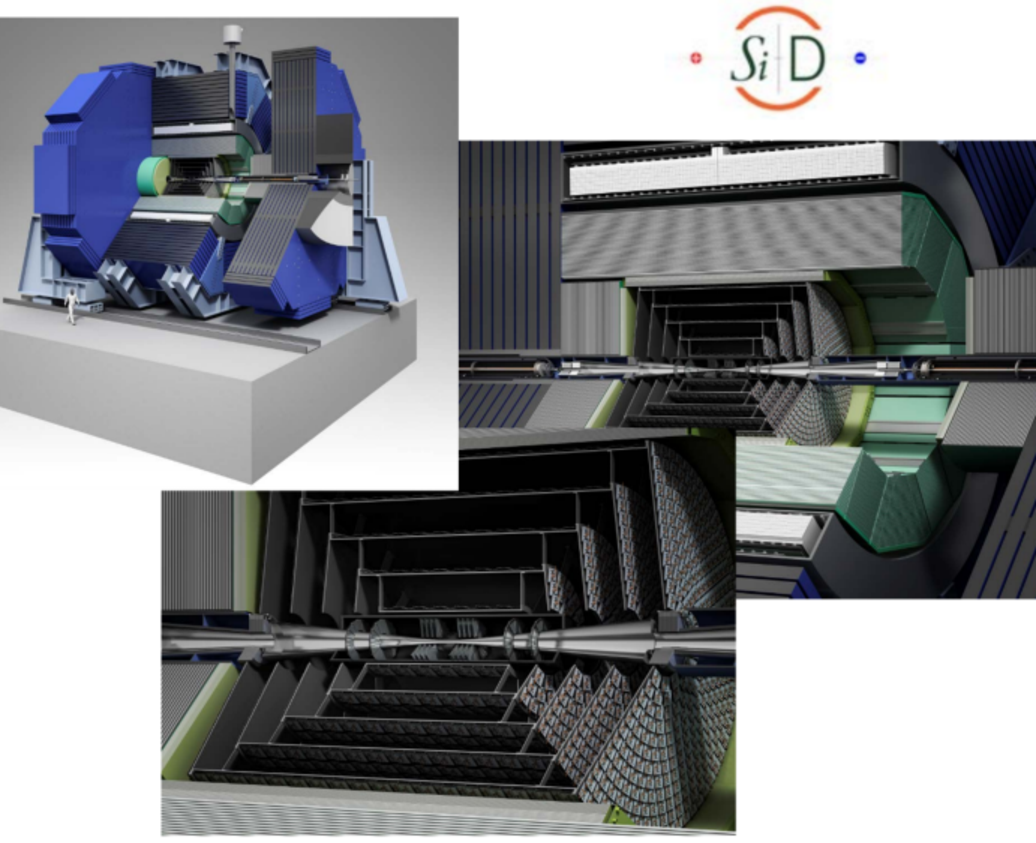
\includegraphics[height=0.4\textheight]{figures/SiDpics.pdf}
 \end{flushright}
  \end{column}
 \end{columns}
\end{frame}

\begin{frame}{SiD detector}
\sidlogo
\begin{figure}[T]
\centering
\begin{subfigure}[b]{0.49\textwidth}
\centering
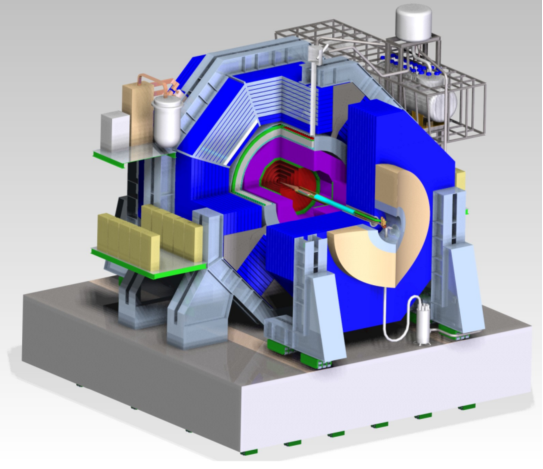
\includegraphics[height=0.65\textheight]{figures/SiD_detector_model.pdf}
\end{subfigure}
\begin{subfigure}[b]{0.49\textwidth}
\centering
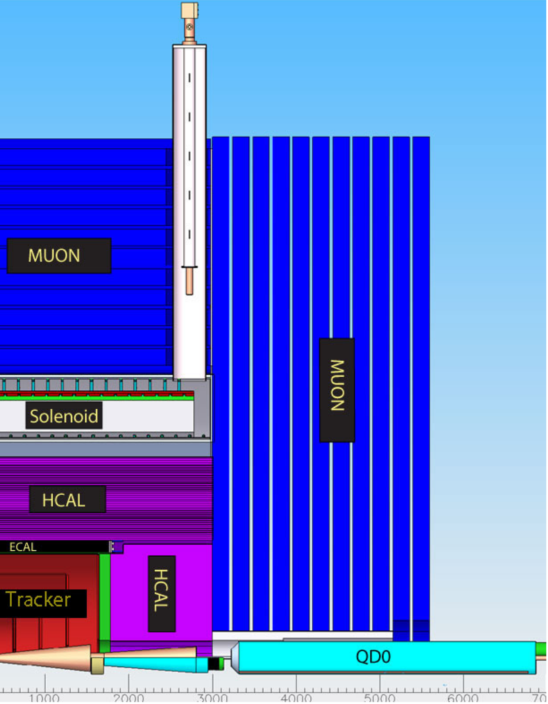
\includegraphics[height=0.65\textheight]{figures/SiD_detector_model_Ausschnitt.pdf}
\end{subfigure}
\end{figure}
{\small SiD detector model: Vertex detector (red), ECAL (green), HCAL (pink), Muon system (blue)}
\end{frame}

\subsection{Background generators}
\sidlogo
\begin{frame}{Generator/Simulation tools}
The background is first modeled with different simulation tools:\\
\begin{itemize}
\item \alert{GuineaPig} (Generator of background events from beam-beam interactions)
\item \alert{BDSIM} (Geant4 based extension toolkit for beam line simulations)
\item \alert{FLUKA} (Fully integrated particle physics MonteCarlo simulation package)
\item \alert{MUCARLO} (Fortran tool to generate muons from the ILC Beam Delivery System)
\end{itemize}
The background events are then simulated in a \alert{full detector simulation} with a Geant4 toolkit.
\begin{figure}
	\begin{columns}
        \column{0.7\linewidth} \flushright
        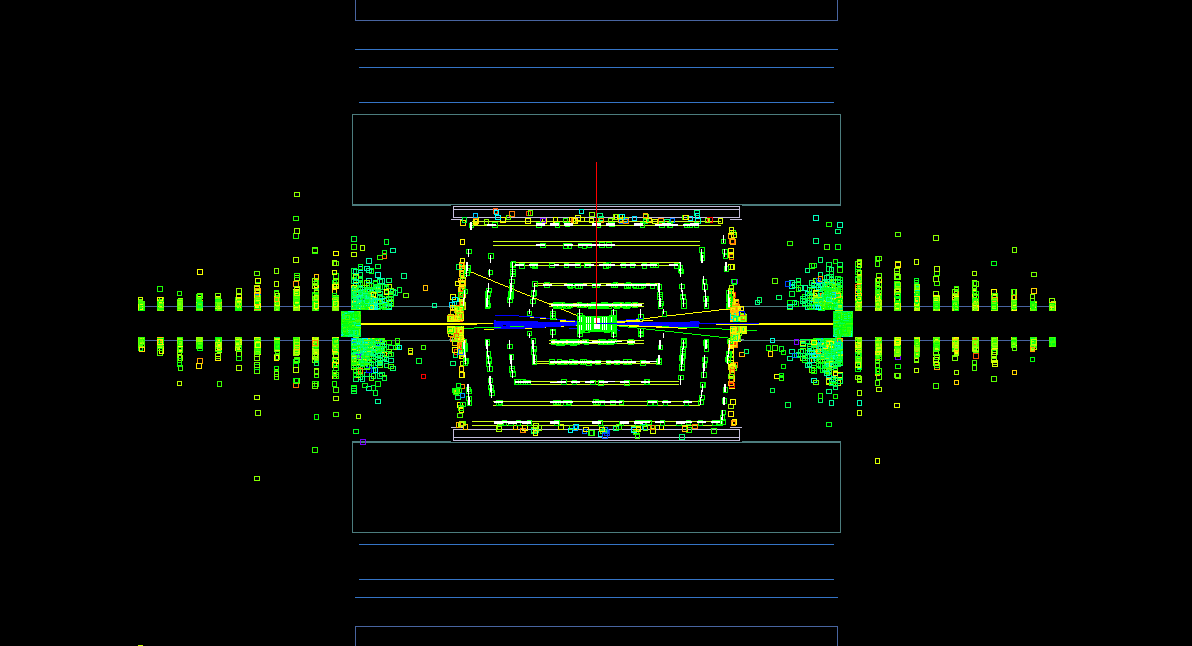
\includegraphics[width=0.61\textwidth]{figures/Full_bunchcrossing_rhoz.png}
        \column{0.3\linewidth}
        {\small The inner detector part of SiD. WIRED4 event display of the pair background of one bunch crossing.}
      \end{columns}
\end{figure}
	
\end{frame}

\begin{frame}{Background sources}
\ilclogo
The main sources of background:
\begin{columns}
 \begin{column}{0.6\textwidth}
  \begin{itemize}
    \item Beam-beam interactions:
    \begin{itemize}
      \item Pair background
      \item Bhabha scattering
      \item \textgamma \textgamma $\rightarrow$ hadrons
    \end{itemize}
    \vspace*{0.5cm}
    \item Machine background:
    \begin{itemize}
      \item Muons from the Beam Delivery System
      \item Background from the Final-Focus system (beam halo collimators)
      \item Neutrons from the Beam Dumps
    \end{itemize}
  \end{itemize}
 \end{column}
 \begin{column}{0.45\textwidth}
 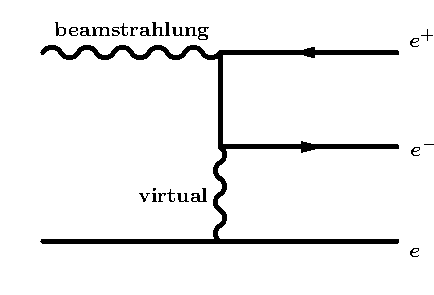
\includegraphics[width=0.33\textwidth]{figures/Bethe-Heitler.pdf}
 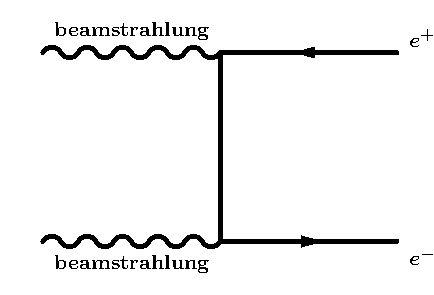
\includegraphics[width=0.33\textwidth]{figures/Breit-Wheeler.pdf}
 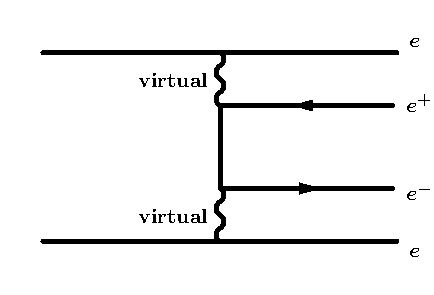
\includegraphics[width=0.33\textwidth]{figures/Landau-Lifshitz.pdf}\\
 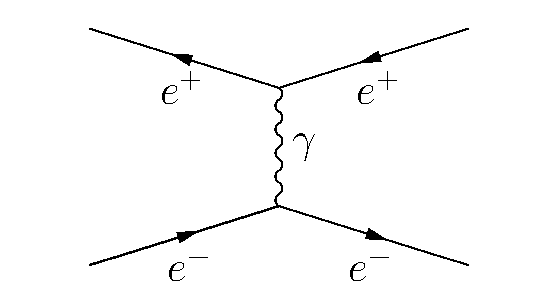
\includegraphics[height=0.15\textheight]{figures/bhabha_scattering.pdf} 
 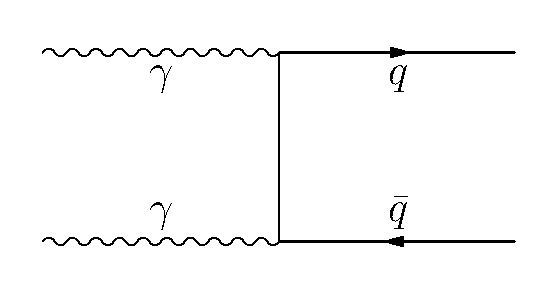
\includegraphics[height=0.15\textheight]{figures/gammagamma_hadrons.pdf}\\
 \vspace*{0.5cm}
 \includegraphics[width=0.8\textwidth]{figures/wall_shielding.png}
 \end{column}
\end{columns}
\end{frame}

\subsection{Pair background}

\begin{frame}{Pair background - Hit time}
\sidlogo
Per bunch, there are about \num{200000} \positron \electron background particles from beam-beam interactions.\\
What is the \textbf{timing} of this important background \textbf{wrt the bunch crossing}?\\\vspace*{0.3cm}
\includegraphics[width=0.52\textwidth]{figures/hittime_SiVertexBarrel.pdf}
\includegraphics[width=0.52\textwidth]{figures/hittime_SiVertexEndcap.pdf}\\
The vertex detector gets hits up to $\sim$ 50ns after the bunch crossing.\\
This is an opportunity to apply \textbf{time gates $\rightarrow$ background reduction!}
\end{frame}
\begin{frame}{Where are these time structures coming from?}
\sidlogo
\only<1>{
\begin{center}
Particle origins of particles hitting the vertex detector in \textcolor{Red}{$[\unit[0]{ns};\unit[10]{ns}]$}
\includegraphics[width=0.7\textwidth]{figures/hitmaps_particleorigins_hittime_histo1_SiVertexEndcapSiVertexBarrel_SiDNote.pdf}
\end{center}
As expected, the pairs originate from the IP and the inner part of the detector.
}
\only<2>{
\begin{center}
Particle origins of particles hitting the vertex detector in \textcolor{Red}{$[\unit[10]{ns};\unit[20]{ns}]$}
\includegraphics[width=0.7\textwidth]{figures/hitmaps_particleorigins_hittime_histo2_SiVertexEndcapSiVertexBarrel_SiDNote.pdf}
\end{center}
The number of hits decreased, but there are still particles originating from the IP.
}
\only<3>{
\begin{center}
Particle origins of particles hitting the vertex detector in \textcolor{Red}{$[\unit[20]{ns};\unit[30]{ns}]$}
\includegraphics[width=0.7\textwidth]{figures/hitmaps_particleorigins_hittime_histo3_SiVertexEndcapSiVertexBarrel_SiDNote.pdf}
\end{center}
The pairs have travelled towards the detector endcaps and have backscattered there.
}
\only<4>{
\begin{center}
Particle origins of particles hitting the vertex detector in \textcolor{Red}{$[\unit[30]{ns};\unit[50]{ns}]$}
\includegraphics[width=0.7\textwidth]{figures/hitmaps_particleorigins_hittime_histo4_SiVertexEndcapSiVertexBarrel_SiDNote.pdf}
\end{center}
The particles still originate from the IP, the detector barrel and the endcaps.
}
\end{frame}

\begin{frame}{Pair background -  P\textsubscript{T}}
\sidlogo
Since their P\textsubscript{T} ranges between 0 and 2\,GeV, they form \textbf{helix tracks in the solenoid field}. The tracks extend to the inner detector layers, and leave up to several tens of hits.
\begin{center}
\includegraphics[width=0.7\textwidth]{figures/PT_hittime_primaries_SiVertexEndcapSiVertexBarrel.pdf}
\end{center}
\end{frame}

\begin{frame}{Pair background envelopes - 500GeV}
%The helix tracks were calculated by a Helix algorithm that I have written.\\
Due to their momentum distributions, the envelopes of all pair background helixes have a characteristic shape.
   \includegraphics[width=0.51\textwidth]{figures/PairHelixes_500GeV_5T_10bunches_xz.png}\hspace*{0.1cm}
   \includegraphics[width=0.51\textwidth]{figures/HelixEnvelopes_Helix_tracks_xz_Helix_in_beampipe_10bunches_500GeV_5T.pdf}\\
The envelopes show that at any given point the beam pipe is 4mm away from 99.9\% of all pair particle tracks.\\
This suggests the possibility to \textbf{reduce the beam pipe and vertex detector radius} by $\sim$2mm.
\end{frame}
%\begin{frame}{Pair background envelopes - 350GeV}
%   \includegraphics[width=0.51\textwidth]{figures/PairHelixes_350GeV_5T.png}\hspace*{0.1cm}
%   \includegraphics[width=0.51\textwidth]{figures/PairEnvelopes_350GeV_5T.png}
%\end{frame}
%\begin{frame}{Pair background envelopes - 250GeV}
%   \includegraphics[width=0.51\textwidth]{figures/PairHelixes_250GeV_5T.png}\hspace*{0.1cm}
%   \includegraphics[width=0.51\textwidth]{figures/PairEnvelopes_250GeV_5T.png}
%\end{frame}

\subsection{Muons from the BDS}

\begin{frame}{The BDS}
\begin{center}
  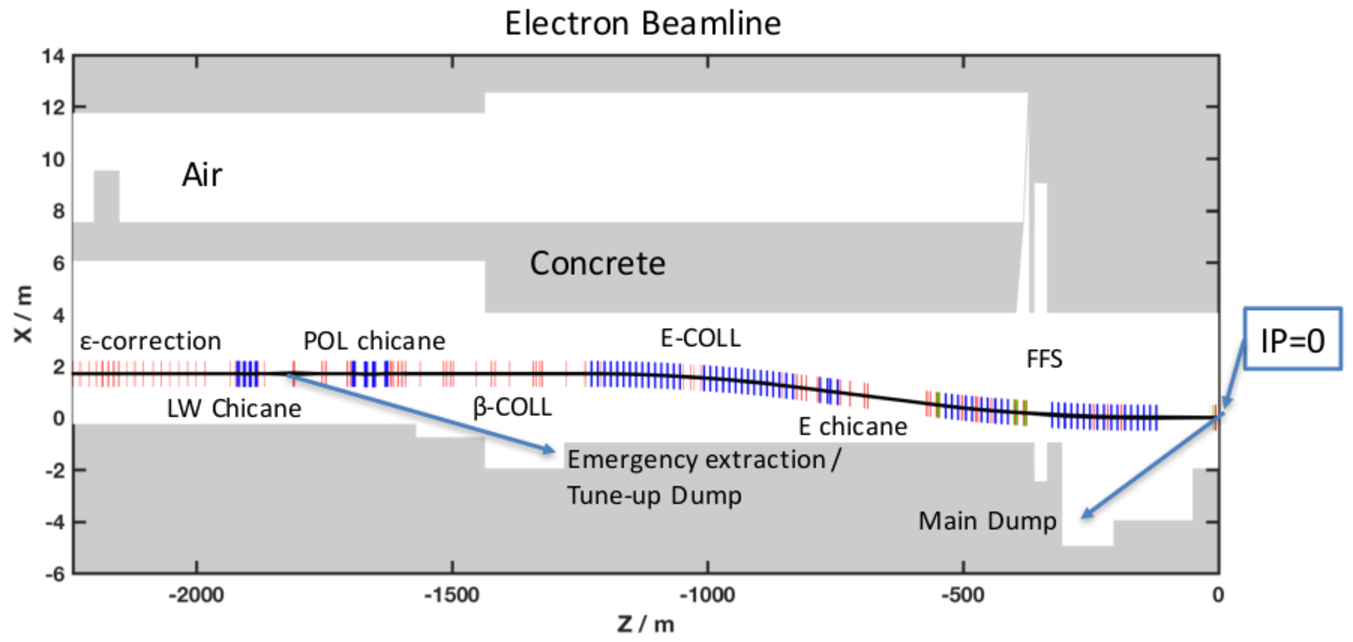
\includegraphics[width=0.9\textwidth]{figures/BDS_electron_tunnel.pdf}
  \end{center}
The Beam Delivery System (BDS) contains the Final Focus System, and therefore focusses the beam on its way to the Interaction Point (IP).
\end{frame}
  \begin{frame}{The BDS}
\begin{center}
  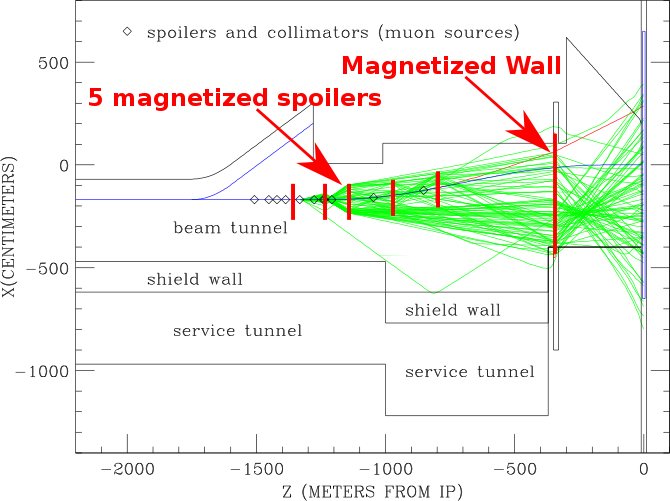
\includegraphics[width=0.7\textwidth]{figures/BDS_Tunnel_Spoilers+Wall.png}
\end{center}
Muons are created along the BDS, when the beam halo interacts with the beam line material.
\end{frame}

\begin{frame}{The Muon Spoilers}
\begin{columns}
 \begin{column}{0.4\textwidth}
 The two suggested shielding scenarios:
  \begin{itemize}
   \item 5 Spoilers
   \begin{itemize}
    \item 70\,cm radius, 5\,m long
    \item magnetized iron
    \item at 5 locations along the BDS
   \end{itemize}
   \item 5 Spoilers + Wall
    \begin{itemize}
    \item 4\,m x 5\,m, 5\,m long
    \item magnetized iron
    \item close to the interaction region
   \end{itemize}
  \end{itemize}

 \end{column}
 \begin{column}{0.6\textwidth}
  \fbox{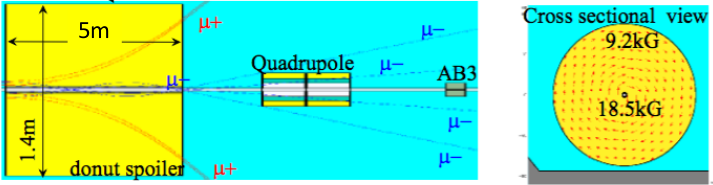
\includegraphics[width=\textwidth]{figures/Spoiler.png}}\\\vspace*{0.3cm}
  \fbox{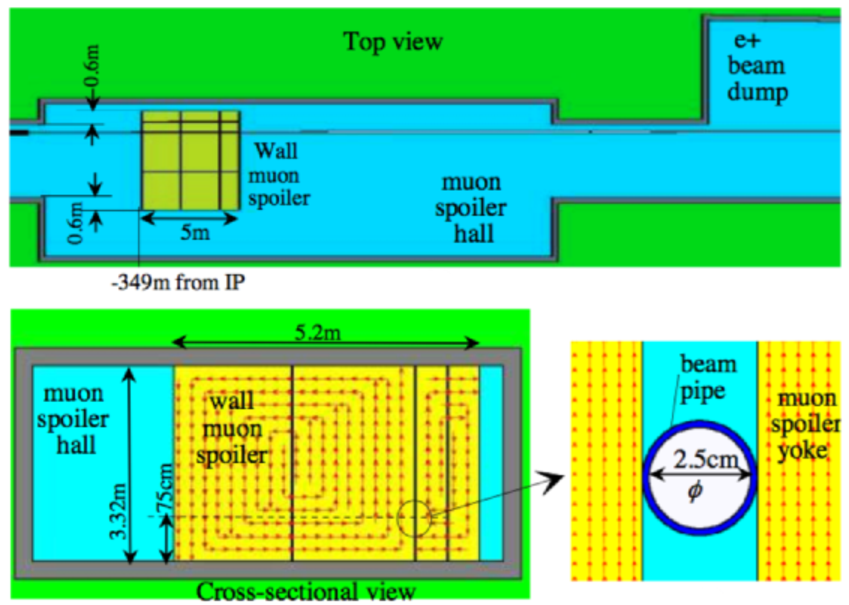
\includegraphics[width=\textwidth]{figures/Muon_wall.pdf}}
 \end{column}
\end{columns} 
\end{frame}

\begin{frame}{WIRED4 event display - 5 Spoilers + Wall}
\sidlogo
1 train's worth of muons ($\sim$ 515 muons) \textbf{from the positron line only}:
\begin{center}
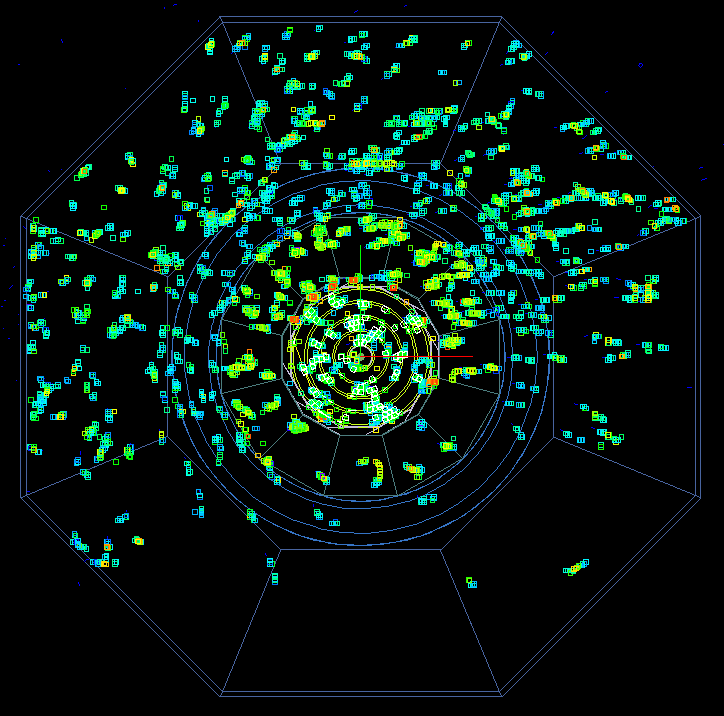
\includegraphics[height=0.6\textheight]{figures/muons_positron_5spoilers_wall_515_xyview_croped.png}
{\tiny xy-view}
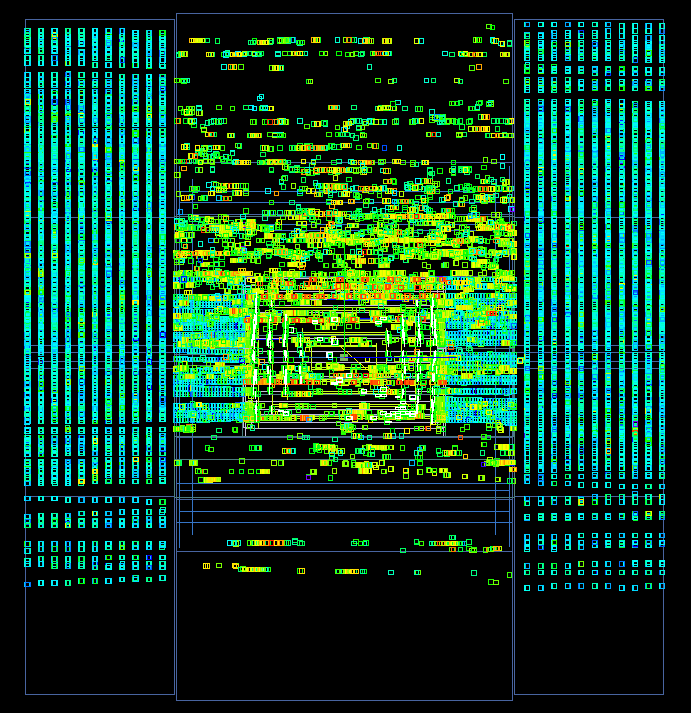
\includegraphics[height=0.6\textheight]{figures/muons_positron_5spoilers_wall_515_zyview_croped.png}
{\tiny zy-view}
\end{center}
Together with the muons from the e\textsuperscript{-} line, there will be \textbf{$\sim$ 900 muons per train in the '5 Spoilers + Wall' scenario}.
\end{frame}
\begin{frame}{WIRED4 event display - 5 Spoilers}
\sidlogo
1 train's worth of muons ($\sim$ 2961 muons) \textbf{from the positron line only}:
\begin{center}
\includegraphics[height=0.6\textheight]{figures/muons_positron_5spoilers_2961_xyview_croped.png}
{\tiny xy-view}
\includegraphics[height=0.6\textheight]{figures/muons_positron_5spoilers_2961_zyview_croped.png}
{\tiny zy-view}
\end{center}
Together with the muons from the e\textsuperscript{-} line, there will be \textbf{$\sim$ 5600 muons per train in the '5 Spoilers' scenario}.\\
The spatial distribution is due to the tunnel shape and its shielding effects.
\end{frame}

\begin{frame}{The Muons in SiD - Spatial Distribution}
 \includegraphics[width=0.9\textwidth]{figures/Explanation_Spatial_distribution_NEW.pdf}
\end{frame}

\begin{frame}{The Muon Occupancy in SiD}
 \includegraphics[width=0.6\textwidth]{figures/Hits_in_SiD_subdetectors_MuonSpoilerStudy.pdf}
  \includegraphics[width=0.45\textwidth]{figures/Explanation_Hits_Subdetectors.pdf}\\
The number of hits in the different SiD subdetectors for both shielding scenarios (\textcolor{Red}{``5 Spoilers''} and \textcolor{Blue}{``5 Spoilers + Wall''}) is not evenly distributed.\\
The number of hits depends on the effective area of the subdetector system.
 \end{frame}
 
\begin{frame}{The Muon Occupancy in SiD ECAL endcaps}
\begin{center}
  \includegraphics[width=0.61\textwidth]{figures/EcalEndcap_DeadCells.png}
\end{center}
{\small A readout cell is ``dead'' when all buffers of the sensor are already filled. No more hits can be stored.}\\
The current SiD electronics design has a \textcolor{Green}{buffer depth of 4}, i.e. \textcolor{Blue}{10\textsuperscript{-6}} - \textcolor{Red}{10\textsuperscript{-4}} of all hits are dead in the ECAL endcaps.
\end{frame}
\begin{frame}
 With the shown results from the occupancy analysis of the muons from the current MUCARLO simulations, the \textbf{SiD group prefers to keep the magnetized wall} in order to keep the occupancy in the SiD detector as low as possible.
 \begin{columns}
  \begin{column}{0.4\textwidth}
    This will also allow access to the detector parking garage, since the wall represents a tertiary containment device against not only muons but also photons and neutrons from the machine background.
  \end{column}
  \begin{column}{0.6\textwidth}
    \includegraphics[width=\textwidth]{figures/wall_shielding.png}
  \end{column}
 \end{columns}
\end{frame}

\subsection{Machine Backgrounds at ATF2}

\begin{frame}{Accelerator Test Facility 2}
\ATFlogo
ATF2
\begin{itemize}
\item Extension of the Accelerator Test Facility (ATF) at KEK in Japan
\item Test bench for the Final-Focus system of the ILC $\rightarrow$ very close to the ILC 500
\item Achieving \SI{42}{\nano\metre} beam size (goal: \SI{39}{\nano\metre})
\end{itemize}
\vspace*{0.3cm}
\begin{center}
 	\includegraphics[width=0.8\textwidth]{figures/ATF.jpg}
\end{center}

\end{frame}

\begin{frame}{Data taking}
\ejadelogo
Thanks to the E-JADE program {\tiny(www.e-jade.eu)}, I was allowed to travel to Japan for participating in the ATF2 beam operation time in March and October 2016.\\
A vertical beam halo collimator was installed by N. Fuster Martinez (IFIC), and its functionallity to reduce the background was to be proven.
\begin{itemize}
\item Operating the ATF beam
\item Studies of the background in the region of the collimator
\end{itemize}
%\vspace*{0.5cm}
\begin{center}
\includegraphics[width=0.65\textwidth]{figures/ATF2_beamhalo_collimator.pdf}
\end{center}
\end{frame}
\begin{frame}{The Vertical Beam Halo Collimator and the\\RHUL Cherenkov detector}
\ATFlogo
\begin{center}
\includegraphics[width=\textwidth]{figures/ATF2schematic.pdf}\\
  \includegraphics[width=\textwidth]{figures/RHUL_detector_Collimator.png}
\end{center}
\end{frame}

\begin{frame}{Background Data taken with the RHUL Cherenkov detector}
\ATFlogo
\begin{center}
 Symmentric jaw movement \hspace*{2.5cm} Jaws moving separately\\
\vspace*{0.2cm}
 \includegraphics[width=0.55\textwidth]{figures/AverageSignal_perAperture.pdf}
  \includegraphics[width=0.55\textwidth]{figures/AverageSignal_perJawPosition_12April2016.pdf}
\end{center}
Background is reduced, but then rises again when collimator jaws are driven closer into the beam halo.\\
Individual jaw movement gives conflicting results.
%\begin{block}{}
%The vertical beam size at the location of the collimator was about \SI{0.32}{mm} with an offset of 0.2-\SI{0.5}{mm}.
%\end{block}
\end{frame}
\begin{frame}{BDSIM simulations of ATF2}
\RHULlogo
\begin{center}
 \includegraphics[width=0.9\textwidth]{figures/atf_bdsim.png}
\end{center}
BDSIM was developed by RHUL: {\small http://www.pp.rhul.ac.uk/bdsim/manual/index.html}\\
BDSIM is a MC simulation tool for simulations of particle accelerators:
\begin{itemize}
 \item C++ program utilising the Geant4 toolkit
 \item simulating the transport of particles in an accelerator
 \item simulating the interaction of particles with the accelerator material
 \item simulating detector backgrounds from the beam halo and machine background sources
 \item Geant4 geometry dynamically and easily built
\end{itemize}
Example applications are background studies for ATF2, CLIC, LHC, ...
\end{frame}

\begin{frame}{BDSIM: Modelling the Vertical Collimator}
\RHULlogo
Collaborating with RHUL to improve BDSIM and the ATF2 geometry model.\\
Any geometry can be modelled and be plugged into BDSIM.
\begin{center}
View inside the collimator model \hspace*{1cm} Collimator in ATF2 beam line\\
\vspace*{0.2cm}
 \includegraphics[width=0.5\textwidth]{figures/Collimator_model.pdf}%\hspace*{1cm}
 \includegraphics[width=0.5\textwidth]{figures/Collimator_in_ATF2.png}
 \end{center}
 Improving the Vertical Collimator model so that the jaws can be placed in any position $\rightarrow$ simulating the different data taking methods
\end{frame}

\begin{frame}{BDSIM: Find places of particle scattering and beam loss}
  \begin{columns}
  \begin{column}{0.3\textwidth}
   Number of secondary particles created in components along the ATF2 beam line
  \end{column}
  \begin{column}{0.7\textwidth}
   \includegraphics[width=1.1\textwidth]{figures/TracksPerModel_firstPart}
  \end{column}
 \end{columns}
\end{frame}


\subsection{Neutrons from the beam dumps}
{
\usebackgroundtemplate{
 \tikz\node[opacity=0.05]{\includegraphics[width=1.1\paperwidth]{figures/TB-0067-300-00-A_stamp.pdf}};
 % \tikz\node[opacity=0.2]{\centering\includegraphics[height=\paperheight]{figures/Iwatecomics.jpg}};
 }
\begin{frame}{FLUKA simulation of the ILC Beam Dump}
\flukalogo
The 16 MW beam is dumped into a water tank after collision.\\Neutrons ($\lesssim$\SI{e10}{\per\square\centi\metre\per\year}) are emitted that radiate the surroundings, and travel back towards the detectors.\\
\vspace*{0.1cm}
%Redoing the simulation studies that were done in 2007, when the design was not decided yet.
Concern about the safety and the functionallity of the beam dump design.
\begin{block}{Simulation step 1}
Simulating the neutrons from the beam dump with FLUKA, using the design drawings by B. Smith~\cite{Smith} to model the dump and the surrounding.
\end{block}

\begin{center}
\includegraphics[height=0.35\textheight]{figures/Front_view_BeamDump_Tomb.png}
\hspace*{0.2cm}
\includegraphics[height=0.35\textheight]{figures/Bird_view_BeamDump_Tomb.png}
\end{center}
\end{frame}

\begin{frame}{FLUKA simulation of the ILC Beam Dump}
\flukalogo
\begin{columns}
\begin{column}[c]{0.4\textwidth}
\includegraphics[height=0.45\textheight]{figures/FLUKA_quadrupole_model.png}\\
\small FLUKA simulation model of one of the ILC EXT lattice quadrupoles.
\end{column}
\begin{column}[c]{0.55\textwidth}
\begin{block}{Simulation step 2}
With Benno List (DESY): Python program to plug the real extraction line lattice into FLUKA.\\
Realistic simulation of the interaction between the neutrons and the lattice.
\end{block}
\begin{block}{Simulation step 3}
Simulating the neutrons reaching the interaction point in a full detector simulation.
\end{block}
\end{column}
\end{columns}
\end{frame}

\begin{frame}{Beam dump simulation goals}
 \flukalogo
 All goals of this study in an overview:
\begin{itemize}
 \item Simulating the neutron flux,
 \item the number of neutrons reaching the IP,
 \item the neutron occupancy in SiD,
 \item the dose of the beam dump surrounding,
 \item the influence of the water composition (amount of deuterium),
 \item the influence of the steel composition of the tank container,
 \item the amount of tritium produced in the water,
 \item the effect of the beam dump design.
\end{itemize}
\vspace*{0.5cm}
\rule{12cm}{.1pt}
\begin{thebibliography}{9}
\setbeamertemplate{bibliography item}[text]
\bibitem{Smith} B. Smith (Rutherford Lab), \emph{Design drawings 0-TB-0067-300-00-A, 0-TB-0067-210-00-A, 0-TB-0067-404-00-A}, Dec. 2006 - Jan. 2007
\end{thebibliography}
\end{frame}
}



\section{Summary and Outlook}
\begin{frame}
\textit{What I have done so far:}
 \begin{itemize} 
  \item Generated \textbf{pair background for 2 full ILC bunch trains} (available on the Grid), wrote a tool for converting GuineaPig output to stdhep or slcio format
  \item Studied the \textbf{timing and origin of pair background and backscattering particles} \textcolor{Green}{$\rightarrow$ possible reduction of background with time gates}
  \item Looked at the \textbf{pair helix envelopes} for 500, 350 and 250GeV ILC staging scenarios \textcolor{Green}{$\rightarrow$ suggested reducing the radius of beam pipe and vertex detector}
  \item Studied two different \textbf{muon shielding possibilies} and the muon occupancy in SiD \textcolor{Green}{$\rightarrow$ Spoilers + magnetized wall is prefered shielding option}
  \item Collaboration with RHUL to \textbf{improve the BDSIM tool and ATF2 geometry model}
  \item \textbf{Modelled the Beam Dump and the EXT line with FLUKA} in collaboration with Benno List (DESY)
  \item \textbf{Successful supervision of two Summer Students} in 2015 and 2016
 \end{itemize}
\end{frame}
\begin{frame}
\textit{What will be done in the next months:}
 \begin{itemize}
  \item Studying the \textbf{occupancy in the vertex detector from the pair background helixes} for different ILC staging scenarios
  \item Finalize the \textbf{BDSIM simulation of ATF2 to compare data to simulation}
  \item \textbf{FLUKA simulations of the neutron fluxes from the beam dump}, through the EXT line, towards the IP
  \item Implement \textbf{PACMAN} (detector shield clamp) in the SiD geometry
 \end{itemize}
\textit{What I also want to do:}
 \begin{itemize}
  \item Put together all simulated background sources to study \textbf{overall background occupancy}
  \item Study possible \textbf{improvement in physics event reconstruction when reducing the beam pipe and vertex detector radius}, whilst looking at the increase in background level at such radii
  \item Vary the ILC running parameters (and redo the background studies) to \textbf{find further limits and requirements for the ILC Final Focus design}
  \item \textbf{Writing up my thesis} in winter 2017/2018
 \end{itemize}
\end{frame}


\section*{The end}
{
\usebackgroundtemplate{
 \tikz\node[opacity=0.1]{\includegraphics[width=\paperwidth,resolution=200]{figures/ilc-Comic.png}};
 % \tikz\node[opacity=0.2]{\centering\includegraphics[height=\paperheight]{figures/Iwatecomics.jpg}};
 }
\begin{frame}
\ilclogo
\begin{center}
If you are interested in SiD and keen on working for the ILC, \\
if you like working in a very international environment, \\
or if you love Japan,\\
there are lots of possible Master's and Ph.D topics.\\
\vspace*{1cm}
\textcolor{RubineRed}{
	\LARGE Thanks!\\
	\begin{CJK}{UTF8}{min}
	どうもありがとうございます。
	\end{CJK}
}
\end{center}
\end{frame}
}

\section*{References}
\begin{thebibliography}{9}
\begin{frame}{References}
\bibitem{TDR} T. Behnke, et al.
\emph{The International Linear Collider - Technical Design Report}, 2013.
\bibitem{LHC TDR} \emph{LHC - Design Report}, \url{http://ab-div.web.cern.ch/ab-div/Publications/LHC-DesignReport.html}
\bibitem{IP beam parameters} ATLAS-CONF-2010-027. \emph{Characterization of Interaction-Point Beam Parameters Using the pp Event-Vertex Distribution Reconstructed in the ATLAS Detector at the LHC}, 2010. \url{http://cds.cern.ch/record/1277659/files/ATLAS-CONF-2010-027.pdf}
\bibitem{ILCPAC2012} M. Peskin. \emph{Physics Motivation for the ILC}, 2012. \url{http://www.fnal.gov/directorate/ILCPAC/2012Dec/Physics-ILCPAC2012-Peskin.pdf}
\end{frame}
\begin{frame}{References}
\bibitem{MIT2013} Klute, Markus, Rémi Lafaye, Tilman Plehn, Michael Rauch, and
Dirk Zerwas. \emph{Measuring Higgs Couplings at a Linear Collider}
EPL (Europhysics Letters) 101, no. 5 (March 1, 2013): 51001. \url{http://dx.doi.org/10.1209/0295-5075/101/51001}
\bibitem{RHUL} Mark Thomson. \emph{Physics and Detectors at the ILC}, 2013. \url{https://www.royalholloway.ac.uk/physics/documents/pdf/events/particlephysicsseminars/13-14markthomson23oct2013.pdf}
\bibitem{ATF2} Kuroda et al. \emph{A plan of KEK-ATF Final Focus Test Beam Line (ATF2)
}. \url{http://icfa-nanobeam.web.cern.ch/icfa-nanobeam/paper/urakawa_ATF2-2.pdf}

\end{frame}
\end{thebibliography}

%--------------------------------------------------------------------------------
\appendix

\begin{frame}
\begin{center}
\LARGE Additional Material
\end{center}
  \tableofcontents
\end{frame}

\section{ILC}
\subsection{ILC parameters}
\begin{frame}{ILC baseline parameters}
\ilclogo
\centering
	\includegraphics[width=\textwidth]{figures/ILCTDR-VOLUME_3-PART_II_ILCparameters.pdf}
\end{frame}
\begin{frame}{ILC parameters for the different upgrade stages}
\ilclogo
\centering
	\includegraphics[width=0.8\textwidth]{figures/ILCTDR-VOLUME_3-PART_II_ILCparametersUpgrades.pdf}
\end{frame}

\subsection{Basic accelerating structure}
\begin{frame}{Basic accelerating structure}
\ilclogo
The main accelerating structures are the two 11km long LINACs.
\begin{itemize}
\item 9-cell superconducting RF cavities operating at 1.3 GHz 
\item Accelerating gradient of >30 MV/m
\item Electrons and positrons accelerated in RF standing waves in the cavities 
\end{itemize}
\begin{center}
\includegraphics[width=0.45\textwidth]{figures/cavity.jpg}
\end{center}
The cavities are also developed, built and tested at DESY.
\end{frame}

\subsection{The Final-Focus system}
\begin{frame}{The Final-Focus system}
 \ilclogo
 The Final-Focus (FF) uses:
\begin{itemize}
 \item Strong compact superconducting quadrupoles to focus the
beam at the IP (single collision point with a 14 mrad beam-crossing angle)
\item Sextupoles providing local chromaticity correction
\item Two superconducting octupole doublets, which use nonlinear
focusing to reduce the amplitude of beam-halo particles while leaving the beam core untouched $\rightarrow$ permitting larger collimation amplitude
\item Collimators and spoilers to prevent the beam halo and background particles from entering the detectors
\end{itemize}
\end{frame}

\section{Pair background}
\subsection{Pair background timing}
\begin{frame}{Creation time of particles hitting the Vertex Detector}
\begin{columns}
 \begin{column}{0.4\textwidth}
Distribution of the time of creation (relative to the instant of the bunch crossing at \unit[0]{ns}) of pair background particles (from 1312 bunches) that hit the endcaps of the vertex detector.
At the time of the bunch crossing about \num{1.6e6} particles are created.\\
{\footnotesize The creation time here is plotted for pair background particles hitting the vertex endcaps only. This is to avoid double counting of particles that would hit both, the barrel and the endcaps.}
 \end{column}
 \begin{column}{0.6\textwidth}
 \includegraphics[width=1.05\textwidth]{figures/creationtime_histo_SiVertexEndcap_SiDNote.pdf}
 \end{column}
\end{columns}
\end{frame}

\begin{frame}{Momentum distribution particles hitting the Vertex Detector}
  \includegraphics[width=0.5\textwidth]{figures/momentum_histo_SiVertexBarrelSiVertexEndcap_SiDNote.pdf}
  \includegraphics[width=0.5\textwidth]{figures/transvmomentum_histo_SiVertexBarrelSiVertexEndcap_SiDNote}\\
  Distributions of the pair background particle momenta of pair background particles from 1312 bunches that will hit the barrel and the endcaps of the vertex detector.
  The plots show the histograms of the total and the transverse momenta of the particles hitting the vertex detector, in certain time intervals.
\end{frame}

\subsection{Pair background helixes}
\begin{frame}{Explanation of helix track calculations}
 \begin{center}
  \includegraphics[width=0.65\textwidth]{figures/Helix_explanation.png}
\end{center}
\end{frame}

\section{Muons from the BDS}
\begin{frame}{The Muon Energy}
\begin{center}
  \includegraphics[width=0.65\textwidth]{figures/muon_energy.pdf}
\end{center}
The energy distribution of the muons from the ``5 Spoilers + Wall'' scenario does not reach the same maximum energy. The muons are decelerated and stopped within the magnetized wall.
\end{frame}

\end{document}
